\documentclass[fleqn, a4paper, 8pt, twoside]{amsart}
\usepackage[extreme, mathdisplays]{savetrees}
\usepackage{exsheets}
\usepackage{amsmath, amssymb, amsthm} %standard AMS packages
\usepackage{marginnote} %marginnotes
\usepackage{gensymb} %miscellaneous symbols
\usepackage{commath} %differential symbols
\usepackage{xcolor} %colours
\usepackage{cancel} %cancelling terms
\usepackage[free-standing-units]{siunitx} %formatting units
\usepackage{tikz, pgfplots} %diagrams
	\usetikzlibrary{calc, hobby, patterns, intersections}
\usepackage{graphicx} %inserting graphics
\usepackage{hyperref} %hyperlinks
\usepackage{datetime} %date and time
\usepackage{ulem} %underline for \emph{}
\usepackage{xfrac, lmodern} %inline fractions
\usepackage{enumerate, enumitem} %numbered lists
\usepackage{float} %inserting floats
\usepackage{tabularx}
\usepackage{titlesec}
\usepackage{microtype}
\usepackage{multicol}
\usepackage{setspace}
\usepackage{breqn}

\titleformat{\part}
	{\titlerule \vspace{0.2ex} \titlerule \vspace{.8ex} \normalfont \bf \huge}{\thepart}{1em}{}[\titlerule \vspace{0.2ex} \titlerule]
\titleformat{\section}
	{\normalfont \bf \LARGE}{\thesection}{1em}{}
\titleformat{\subsection}
	{\normalfont \bf \Large}{\thesubsection}{1em}{}

%\renewenvironment{question}{\begin{question}\color{red}}{%
%    \end{question}\ignorespacesafterend
%}

\setlength{\belowcaptionskip}{-10pt}
\allowdisplaybreaks[4]

\newcommand\numberthis{\addtocounter{equation}{1}\tag{\theequation}} %adds numbers to specific equations in non-numbered list of equations

\newcommand{\AxisRotator}[1][rotate=0]{
	\tikz [x=0.25cm,y=0.60cm,line width=.2ex,-stealth,#1] \draw (0,0) arc (-150:150:1 and 1);%
} %rotation symbols on axes

\newtheoremstyle{redtheorem}
{}
{}
{\itshape}
{}
{\color{red}\bfseries}
{}
{ }
{}

\newtheoremstyle{greendefinition}
{}
{}
{\color{green}}
{}
{\color{green}\bfseries}
{}
{ }
{}

\newtheoremstyle{bluedefinition}
{}
{}
{}
{}
{\color{blue}\bfseries}
{}
{ }
{}

\theoremstyle{definition}
\newtheorem{example}{Example}

\theoremstyle{bluedefinition}
\newtheorem{definition}{Definition}

\theoremstyle{redtheorem}
\newtheorem{theorem}{Theorem}

\newcommand{\curl}{\mathrm{curl\,}}

\newcommand{\divergence}{\mathrm{div\,}}

\makeatletter
\@addtoreset{section}{part} %resets section numbers in new part
\makeatother

\makeatletter
\newcommand*{\relrelbarsep}{.386ex}
\newcommand*{\relrelbar}{%
  \mathrel{%
    \mathpalette\@relrelbar\relrelbarsep
  }%
}
\newcommand*{\@relrelbar}[2]{%
  \raise#2\hbox to 0pt{$\m@th#1\relbar$\hss}%
  \lower#2\hbox{$\m@th#1\relbar$}%
}
\providecommand*{\rightrightarrowsfill@}{%
  \arrowfill@\relrelbar\relrelbar\rightrightarrows
}
\providecommand*{\leftleftarrowsfill@}{%
  \arrowfill@\leftleftarrows\relrelbar\relrelbar
}
\providecommand*{\xrightrightarrows}[2][]{%
  \ext@arrow 0359\rightrightarrowsfill@{#1}{#2}%
}
\providecommand*{\xleftleftarrows}[2][]{%
  \ext@arrow 3095\leftleftarrowsfill@{#1}{#2}%
}
\makeatother

\newcommand\blfootnote[1]{%
	\begingroup
	\renewcommand\thefootnote{}\footnote{#1}%
	\addtocounter{footnote}{-1}%
	\endgroup
}

\SetupExSheets{solution/print = true} %prints all solutions by default
%opening
\title{\Huge Differential and Integral Calculus}
\author{Aakash Jog}
\date{\formatdate{3}{7}{2015}}

\begin{document}

\maketitle

\setlength{\mathindent}{0pt}

\begin{multicols}{2}

\begin{spacing}{0.7}

\part{Sequences and Series}

\section{Sequences}

\begin{definition}[Sequences bounded from above]
	$\{a_n\}$ is said to be bounded from above if $\exists M \in \mathbb{R}$, s.t. $a_n \leq M$, $\forall n \in \mathbb{N}$.
	Each such $M$ is called an upper bound of $\{a_n\}$.
\end{definition}

\begin{definition}[Sequences bounded from below]
	$\{a_n\}$ is said to be bounded from below if $\exists m \in \mathbb{R}$, s.t. $a_n \geq M$, $\forall n \in \mathbb{N}$.
	Each such $M$ is called an lower bound of $\{a_n\}$.
\end{definition}

\begin{definition}
	$\{a_n\}$ is said to be bounded if it is bounded from below and bounded from above.
\end{definition}

\begin{definition}[Monotonic increasing sequence]
	A sequence $\{a_n\}$ is called monotonic increasing if $\exists n_0 \in \mathbb{N}$, s.t. $a_n \leq a_{n + 1}$, $\forall n \geq n_0$.
\end{definition}

\begin{definition}[Monotonic decreasing sequence]
	A sequence $\{a_n\}$ is called monotonic decreasing if $\exists n_0 \in \mathbb{N}$, s.t. $a_n \geq a_{n + 1}$, $\forall n \geq n_0$.
\end{definition}

\begin{definition}[Strongly increasing sequence]
	A sequence $\{a_n\}$ is called monotonic increasing if $\exists n_0 \in \mathbb{N}$, s.t. $a_n < a_{n + 1}$, $\forall n \geq n_0$.
\end{definition}

\begin{definition}[Strongly decreasing sequence]
	A sequence $\{a_n\}$ is called monotonic decreasing if $\exists n_0 \in \mathbb{N}$, s.t. $a_n > a_{n + 1}$, $\forall n \geq n_0$.
\end{definition}

\subsection{Limit of a Sequence}

\begin{definition}[Limit of a sequence]
	Let $\{a_n\}$ be a given sequence.
	A number $L$ is said to be the limit of the sequence if $\forall \varepsilon > 0$, $\exists n_0 \in \mathbb{N}$, s.t. $|a_n - L| < \varepsilon$, $\forall n \geq n_0$.
	That is, there are infinitely many terms inside the interval and a finite number of terms outside it.
\end{definition}

\begin{question}
	Prove that 2 is not a limit of $\left\{ \frac{3n + 1}{n} \right\}$.
\end{question}

\begin{solution}
	If possible, let 
	\begin{align*}
		\lim\limits_{n \to \infty} \frac{3n + 1}{n} = 2
	\end{align*}
	Then, $\forall \varepsilon > 0$, $\exists n_0 \in \mathbb{N}$, s.t. $\left| \frac{3n + 1}{n} - 2 \right| < \varepsilon$, $\forall n \geq n_0$.
	However,
	\begin{equation*}
		\left| \frac{3n + 1}{n} - 2 \right| = 1 + \frac{1}{n} > 1
	\end{equation*}
	This is a contradiction for $\varepsilon = \frac{1}{2}$.
	Therefore, 2 is not a limit.
\end{solution}

\begin{theorem}
	If a sequence $\{a_n\}$ has a limit $L$ then the limit is unique.
	\label{uniquness of a limit}
\end{theorem}

\begin{theorem}
	If a sequence $\{a_n\}$ has limit $L$, then the sequence is bounded.
	\label{existence of limit implies boundedness}
\end{theorem}

\begin{theorem}
	Let
	\begin{align*}
		\lim\limits_{n \to \infty} a_n &= a\\
		\lim\limits_{n \to \infty} b_n &= b
	\end{align*}
	and let $c$ be a constant.
	Then,
	\begin{align*}
		\lim c &= c\\
		\lim (c a_n) &= c \lim a_n\\
		\lim (a_n \pm b_n) &= \lim a_n \pm \lim b_n\\
		\lim (a_n b_n) &= \lim a_n \lim b_n\\
		\lim (\frac{a_n}{b_n}) &= \frac{\lim a_n}{\lim b_n} \quad (\textnormal{ if } \lim b \neq 0)
	\end{align*}
	\label{limit arithmetic}
\end{theorem}

\begin{theorem}
	Let $\{b_n\}$ be bounded and let $\lim a_n = 0$. Then,
	\begin{equation*}
		\lim (a_n b_n) = 0
	\end{equation*}
\end{theorem}

\begin{theorem}[Sandwich Theorem]
	Let $\{a_n\}$, $\{b_n\}$, $\{c_n\}$ be three sequences. If
	\begin{equation*}
		\lim a_n = \lim b_n = L
	\end{equation*}
	and $\exists n_0 \in \mathbb{N}$, s.t. $\forall n \geq n_0$, $a_n \leq b_n \leq c_n$.
	Then,
	\begin{equation*}
		\lim b_n = L
	\end{equation*}
	\label{sandwich theorem}
\end{theorem}

\begin{question}
	Calculate $\lim\limits_{n \to \infty} \sqrt[n]{2^n + 3^n}$
\end{question}

\begin{solution}[print]
	\begin{gather*}
		\sqrt[n]{3^n} \leq \sqrt[n]{2^n + 3^n} \leq \sqrt[n]{3^n + 3^n} = \sqrt[3]{2 \cdot 3^n}\\
		\therefore 3 \leq \sqrt[n]{2^n + 3^n} \leq 3 \sqrt[n]{2}
	\end{gather*}
	Therefore, by the \nameref{sandwich theorem}, $\lim\limits_{n \to \infty} \sqrt[n]{2^n + 3^n} = 3$.
\end{solution}

\begin{theorem}
	Any monotonically increasing sequence which is bounded from above converges.
	Similarly, any monotonically decreasing sequence which is bounded from below converges.
	\label{monotonicity and boundedness implies convergence}
\end{theorem}

\begin{question}
	Prove that there exists a limit for $a_n = \underbrace{\sqrt{2 + \sqrt{2 + \sqrt{2 + \dots}}}}_{n \textnormal{ times }}$ and find it.
\end{question}

\begin{solution}[print]
	\begin{equation*}
		a_1 = \sqrt{2} < \sqrt{2 + \sqrt{2}} = a_2
	\end{equation*}
	If possible, let
	\begin{align*}
		a_{n - 1} &< a_n\\
		\therefore \sqrt{2 + a_{n - 1}} &< \sqrt{2 + a_n}\\
		\therefore a_n &< a_{n + 1}
	\end{align*}
	Hence, by induction, $\{a_n\}$ is monotonically increasing.
	~\\
	\begin{equation*}
		a_1 = \sqrt{2} \leq 2
	\end{equation*}
	If possible, let
	\begin{align*}
		a_n &\leq 2\\
		\therefore \sqrt{2 + a_n} &\leq \sqrt{2 + 2}\\
		\therefore a_{n + 1} \leq 2
	\end{align*}
	Hence, by induction, $\{a_n\}$ is bounded from above by 2.
	Therefore, by \nameref{monotonicity and boundedness implies convergence}, $\{a_n\}$ converges.
\end{solution}

\subsection{Sub-sequences}

\begin{definition}[Sub-sequence]
	Let $\{a_n\}_{n = 1} ^{\infty}$ be a sequence.
	Let $\{n_k\}_{k = 1}^{\infty}$ be a strongly increasing sequence of natural numbers.
	Let $\{b_k\}_{k = 1}^{\infty}$ be a sequence such that $b_k = a_{n_k}$.
	Then $\{b_k\}_{k = 1}^{\infty}$ is called a sub-sequence of $\{a_n\}_{n = 1}^{\infty}$.
\end{definition}

\begin{theorem}
	If the sequence $\{a_n\}$ converges to $L$ in a wide sense, i.e. $L$ can be infinite, then any sub-sequence of $\{a_n\}$ converges to the same limit $L$.
	\label{Any subsequence converges to the limit of the sequence}
\end{theorem}

\begin{definition}[Partial limit]
	A real number $a$, which may be infinite, is called a partial limit of the sequence $\{a_n\}$ is there exists a sub-sequence of $\{a_n\}$ which converges to $a$.
\end{definition}

\begin{theorem}[Bolzano-Weierstrass Theorem]
	For any bounded sequence there exists a subsequence which is convergent, s.t. there exists at least one partial limit.
	\label{Bolzano-Weierstrass Theorem}
\end{theorem}

\begin{definition}[Upper partial limit]
	The largest partial limit of a sequence is called the upper partial limit.
	It is denoted by $\overline{\lim} a_n$ or $\limsup a_n$.
\end{definition}

\begin{definition}[Lower partial limit]
	The smallest partial limit of a sequence is called the upper partial limit.
	It is denoted by $\underline{\lim} a_n$ or $\liminf a_n$.
\end{definition}

\begin{theorem}
	If the sequence $\{a_n\}$ is bounded and $\overline{\lim} a_n = \underline{\lim} a_n = a$ then $\exists \lim a_n = a$.
	\label{Equal upper and lower partial limits imply existence of limit}
\end{theorem}

\subsection{Cauchy Characterisation of Convergence}

\begin{definition}
	A sequence $\{a_n\}$ is called a Cauchy sequence if $\forall \varepsilon > 0$, $\exists n_0 \in \mathbb{N}$, s.t. $\forall m, n \geq n_0$, $|a_n - a_m| < \varepsilon$.
\end{definition}

\begin{theorem}[Cauchy Characterisation of Convergence]
	A sequence $\{a_n\}$ converges if and only if it is a Cauchy sequence.
	\label{Cauchy Characterisation of Convergence}
\end{theorem}

\begin{theorem}[Another Formulation of the Cauchy Characterisation Theorem]
	The sequence $\{a_n\}$ converges if and only if $\forall \varepsilon > 0$, $\exists n_0 \in \mathbb{N}$, such that $\forall n \geq n_0$ and $\forall p \in \mathbb{N}$, $|a_{n + p} - a_n| < \varepsilon$.
	\label{Another formulation of the Cauchy characterisation theorem}
\end{theorem}

\begin{question}
	Prove that the sequence $a_n = \frac{1}{1^2} + \frac{1}{2^2} + \dots + \frac{1}{n^2}$ is convergent.
\end{question}

\begin{solution}
	\begin{align*}
		|a_{n + p} - a_n| &= \left| \frac{1}{1^2} + \frac{1}{2^2} + \dots + \frac{1}{(n + p)^2} - \left( \frac{1}{1^2} + \frac{1}{2^2} + \dots + \frac{1}{n^2} \right) \right|\\
		&= \frac{1}{(n + 1)^2} + \frac{1}{(n + 2)^2} + \dots + \frac{1}{(n + p)^2}\\
		\therefore |a_{n + p} - a_n| &< \frac{1}{n (n + 1)} + \frac{1}{(n + 1)(n + 2)} + \dots + \frac{1}{(n + p - 1)(n + p)}\\
		\therefore |a_{n + p} - a_n| &< \frac{1}{n} - \cancel{\frac{1}{n + 1}} + \cancel{\frac{1}{n + 1}} + \dots + \cancel{\frac{1}{n + p - 1}} - \frac{1}{n + p}\\
		\therefore |a_{n + p} - a_n| &< \frac{1}{n} - \frac{1}{n + p}\\
		\therefore |a_{n + p} - a_n| &< \frac{1}{n}
	\end{align*}
	Therefore, $\forall \varepsilon > 0$, $\exists n_0 \in \mathbb{N}$, s.t. $\forall n \geq n_0$ and $\forall p \in \mathbb{N}$, $|a_{n + p} - a_n| < \varepsilon$, where $n_0 > \frac{1}{\varepsilon}$.
	\qed
\end{solution}

\begin{question}
	Prove that the sequence
	\begin{equation*}
		a_n = \frac{1}{1} + \frac{1}{n} + \dots + \frac{1}{n}
	\end{equation*}
	diverges.
\end{question}

\begin{solution}
	If possible, let the sequence converge.
	Then, by the \nameref{Cauchy Characterisation of Convergence}, $\forall \varepsilon > 0$, $\exists n_0 \in \mathbb{N}$, s.t. $\forall n \geq n_0$ and $\forall p \in \mathbb{N}$, $|a_{n + p} - a_n| < \varepsilon$.\\
	Therefore,
	\begin{align*}
		|a_{n + p} - a_n| &= \left| \frac{1}{1} + \frac{1}{2} + \dots + \frac{1}{n} + \frac{1}{n + p} - \left( \frac{1}{n} + \dots + \frac{1}{n} \right) \right|\\
		&= \frac{1}{n + 1} + \dots + \frac{1}{n + p}\\
		&\ge p \cdot \frac{1}{n + p}\\
		\therefore |a_{n + p} - a_n| &> \frac{p}{n + p}
	\end{align*}
	If $n = p$,
	\begin{align*}
		\frac{p}{n + p} &= \frac{1}{2}
	\end{align*}
	This contradicts the result obtained from the \nameref{Cauchy Characterisation of Convergence}, for $\varepsilon = \frac{1}{4}$.\\
	Therefore, the sequence diverges.
\end{solution}

\section{Series}

\begin{definition}[$p$-series]
	The series $\sum\limits_{n = 1}^{\infty} \frac{1}{n^p}$ is called the $p$-series.
\end{definition}

\begin{theorem}
	The $p$-series converges for $p > 1$ and diverges for $p \le 1$.
	\label{convergence and divergence of p-series}
\end{theorem}

\begin{theorem}
	If $\sum a_n$ converges, then $\lim\limits_{n \to \infty} a_n = 0$, but the converse is not true.
\end{theorem}

\begin{theorem}
	If $\sum a_n$ and $\sum b_n$ converge, then $\sum (a_n \pm b_n)$ and $\sum c a_n$, where $c$ is a constant, also converge. Also,
	\begin{align*}
		\sum (a_n \pm b_n) &= \sum a_n \pm \sum b_n\\
		\sum (c a_n) &= c \sum a_n
	\end{align*}
\end{theorem}

\subsection{Convergence Criteria}

\subsubsection{Leibniz's Criteria}

\begin{theorem}[Leibniz's Criteria for Convergence]
	If an alternating series $\sum (-1)^{n - 1} a_n$ with $a_n > 0$ satisfies
	\begin{enumerate}
		\item $a_{n + 1} \le a_n$, i.e. $\{a_n\}$ is monotonically decreasing.
		\item $\lim\limits_{n \to \infty} a_n = 0$
	\end{enumerate}
	then the series $(-1)^{n - 1} a_n$ converges.
	\label{Leibniz's Criteria for Convergence}
\end{theorem}

\begin{example}
	The alternating harmonic series $\sum \frac{(-1)^{n - 1}}{n}$ converges as $a_n = \frac{1}{n} > 0$, $a_n$ decreases and $\lim a_n = 0$.
\end{example}

\subsubsection{Comparison Test}

\begin{theorem}[First Comparison Test for Convergence]
	Assume $\exists n_0 \in \mathbb{N}$, such that $a_n \ge 0$, $b_n \ge 0$, $\forall n \ge n_0$.
	\begin{enumerate}
		\item If $a_n \le b_n$, $\forall n \ge n_0$ and $\sum\limits_{n = 1}^{\infty} b_n$ converges, then $\sum\limits_{n = 1}^{\infty} a_n$ converges.
		\item If $a_n \ge b_n$, $\forall n \ge n_0$ and $\sum\limits_{n = 1}^{\infty} b_n$ diverges, then $\sum\limits_{n = 1}^{\infty} a_n$ diverges.
	\end{enumerate}
\end{theorem}

\begin{theorem}[Another Formulation of the Comparison Test for Convergence]
	Assume $\exists n_0 \in \mathbb{N}$, such that $a_n \ge 0$, $b_n \ge 0$, $\forall n \ge n_0$, then if $\lim\limits_{n \to \infty} \frac{a_n}{b_n}$ exists, then $\sum a_n$ and $\sum b_n$ converge or diverge simultaneously.
\end{theorem}

\subsubsection{d'Alembert Criteria (Ratio Test)}

\begin{definition}[Absolute and conditional convergence]
	The series $\sum a_n$ is said to converge absolutely if $\sum |a_n|$ converges.
	The series $\sum a_n$ is said to converge conditionally if it converges but $\sum |a_n|$ diverges.
\end{definition}

\begin{theorem}
	If the series $\sum a_n$ converges absolutely then it converges.
\end{theorem}

\begin{theorem}[d'Alembert Criteria (Ratio Test)]
	\begin{enumerate}
		\item 
			If $\lim\limits_{n \to \infty} \left| \frac{a_{n + 1}}{a_n} \right| = L < 1$ then $\sum a_n$ converges absolutely.
		\item 
			If $\lim\limits_{n \to \infty} \left| \frac{a_{n + 1}}{a_n} \right| = L > 1$(including $L = \infty$), then $\sum a_n$ converges diverges.
		\item
			If $L = 1$, the test does not apply.
	\end{enumerate}
	\label{d'Alembert Criteria (Ratio Test)}
\end{theorem}

\subsubsection{Cauchy Criteria (Cauchy Root Test)}

\begin{theorem}[Cauchy Criteria (Cauchy Root Test)]
	\begin{enumerate}
		\item
			If $\overline{\lim} \sqrt[n]{|a_n|} = L < 1$ then $\sum a_n$ converges absolutely.
		\item
			If $\overline{\lim} \sqrt[n]{|a_n|} = L > 1$ (including $L = \infty$), then $\sum a_n$ diverges.
		\item
			If $L = 1$, the test does not apply.
	\end{enumerate}
	\label{Cauchy Criteria (Cauchy Root Test)}
\end{theorem}

\subsubsection{Integral Test}

\begin{theorem}[Integral Test for Series Convergence]
	Let $f(x)$ be a continuous, non-negative, monotonic decreasing function on $[1,\infty)$ and let $a_n = f(n)$.
	Then the series $\sum\limits_{n = 1}^{\infty} a_n$ converges if and only if the improper integral $\int\limits_{1}^{\infty} f(x) \dif x$ converges.
	\label{Integral Test for Series Convergence}
\end{theorem}

\begin{theorem}
	If the series $\sum a_n$ absolutely converges and the series $\sum b_n$ is obtained from $\sum a_n$ by changing the order of the terms in $\sum a_n$ then $\sum b_n$ also absolutely converges and $\sum b_n = \sum a_n$.
\end{theorem}

\begin{theorem}
	If a series converges then the series with brackets without changing the order of terms also converges.
	That is, if $\sum a_n$ converges, then any series of the form $(a_1 + a_2) + (a_3 + a_4 + a_5) + a_6 + \dots$ also converges.
\end{theorem}

\begin{theorem}
	If a series with brackets converges and the terms in the brackets have the same sign, then the series without brackets also converges.
\end{theorem}

\section{Power Series}

\begin{definition}[Power series]
	The series $\sum\limits_{n = 0}^{\infty} a_n (x - c)^n$ is called a power series.
\end{definition}

\begin{theorem}[Cauchy-Hadamard Theorem]
	For any power series $\sum\limits_{n = 0}^{\infty} a_n (x - c)^n$ there exists the limit, which may be infinity, $R = \frac{1}{\overline{\lim\limits_{n \to \infty}} \sqrt[n]{|a_n|}}$	and the series converges for $|x - c| < R$ and diverges for $|x - c| > R$.
	The end points of the interval, i.e. $x = c - R$ and $x = c + R$ must be separately checked for series convergence.
\end{theorem}

\begin{definition}[Radius of convergence and convergence interval]
	The number $R$ is called the radius of convergence and the interval $|x - c| < R$ is called the convergence interval of the series.
	The point $c$ is called the centre of the convergence interval.
\end{definition}

\begin{theorem}
	If $\exists \lim\limits_{n \to \infty} \left| \frac{a_n}{a_{n + 1}} \right|$, which may be infinite, then, $R = \lim\limits_{n \to \infty} \left| \frac{a_n}{a_{n + 1}} \right|$.
\end{theorem}

\begin{theorem}[Stirling's Approximation]
	For $n \to \infty$, $n! \approx \left( \frac{n}{e} \right)^n \sqrt{2 \pi n}$.
\end{theorem}

\begin{question}
	Find the domain of convergence of $\sum\limits_{n = 1}^{\infty} \dfrac{(2x - 4)^n}{n}$.
\end{question}

\begin{solution}
	\begin{align*}
		\sum_{n = 1}^{\infty} \dfrac{(2x - 4)^n}{n} &= \sum_{n = 1}^{\infty} \dfrac{2^n (x - 2)^n}{n}
	\end{align*}
	Therefore, by Cauchy's Formula for Radius of Convergence,
	\begin{align*}
		R &= \dfrac{1}{\overline{\lim} \sqrt[n]{|a_n|}}\\
		&= \dfrac{1}{\lim\limits_{n \to \infty} \sqrt[n]{\dfrac{2^n}{n}}}\\
		&= \dfrac{1}{\lim\limits_{n \to \infty} \dfrac{2}{\sqrt[n]{n}}}\\
		&= \dfrac{1}{2}
	\end{align*}
	Therefore, the series converges for
	\begin{equation*}
		|x - 2| < \dfrac{1}{2}
	\end{equation*}
	and diverges for
	\begin{equation*}
		|x - 2| > \dfrac{1}{2}
	\end{equation*}
	If $x = \dfrac{5}{2}$, 
	\begin{align*}
		\sum_{n = 1}^{\infty} \dfrac{2^n}{n} \left( \dfrac{5}{2} - 2 \right)^n\\
		&= \sum_{n = 1}^{\infty} \dfrac{1}{n}
	\end{align*}
	Therefore, the series diverges.\\
	If $x = \dfrac{3}{2}$, 
	\begin{align*}
		\sum_{n = 1}^{\infty} \dfrac{2^n}{n} \left( \dfrac{3}{2} - 2 \right)^n\\
		&= \sum_{n = 1}^{\infty} (-1)^n \dfrac{1}{n}
	\end{align*}
	Therefore, by Leibniz's Criteria for Convergence, the series converges.\\
	Therefore, the domain of convergence is $\left[ \dfrac{3}{2} , \dfrac{5}{2} \right)$.
\end{solution}

\begin{question}
	Find the radius of convergence of $\sum\limits_{n = 0}^{\infty} n! x^{n!}$.
\end{question}

\begin{solution}
	\begin{align*}
		\dfrac{1}{\overline{\lim}\sqrt[n]{a_n}} &= x + x + 2 x^2 + 6 x^6 + 24 x^{24} + \dots
	\end{align*}
	Therefore,
	\begin{align*}
		a_n &=
			\begin{cases}
				n &;\quad n = k^2\\
				0 &;\quad n \neq k^2\\
			\end{cases}
	\end{align*}
	Therefore, 
	\begin{align*}
		R &= \dfrac{1}{\lim\limits_{n \to \infty} \sqrt[n]{a_n}}\\
		&= \dfrac{1}{\lim\limits_{k \to \infty} \sqrt[k!]{k!}}\\
		&= 1
	\end{align*}
\end{solution}

\section{Series of Real-valued Functions}

\begin{definition}[Sequence of functions]
	A sequence $\{f_n\} = f_1(x), f_2(x), \dots$ defined on $D \subseteq \mathbb{R}$ is called a sequence of functions.
\end{definition}

\begin{definition}[Pointwise convergence and domain of convergence]
	$\{f_n\}$ converges pointwise in some domain $E \subseteq D$ if for every $x \in E$, the sequence of $\{f_n(x)\}$ converges.
	In such a case, $E$ is said to be a domain of convergence of $\{f_n\}$.
\end{definition}

\begin{question}
	Find the domain of convergence of $f_n(x) = x^n$, defined on some $D \subseteq \mathbb{R}$.
\end{question}

\begin{solution}
	\begin{align*}
		\lim\limits_{n \to \infty} f_n(x) &= 
			\begin{cases}
				0               & ;\quad -1 < x < 1      \\
				1               & ;\quad x = 1           \\
				\text{diverges} & ;\quad x \notin (-1,1] \\
			\end{cases}
	\end{align*}
	Therefore, the domain of convergence of $\{f_n\}$ is $(-1,1]$.
\end{solution}

\begin{question}
	Let $f(x) : (0,\infty) \to \mathbb{R}$ be some function such that $\lim\limits_{x \to \infty} f(x) = 0$.
	Let $f_n(x) = f(n x)$.
	What is the domain of convergence of $f_n$?
	What is the limit function?
\end{question}

\begin{solution}
	Let $x$ have some fixed value in $(0,\infty)$.
	Therefore, as $\lim\limits_{x \to \infty} f(x) = 0$,
	\begin{align*}
		\lim\limits_{n \to \infty} f_n(x) & = \lim\limits_{n \to \infty} f(n x) \\
                                                  & = 0
	\end{align*}
	Therefore, the domain of convergence is $(0,\infty)$ and the limit function is a constant function with value $0$.
\end{solution}

\subsection{Uniform Convergence of Series of Functions}

\begin{definition}[Pointwise convergence of a sequence of functions]
	If $\forall x \in D$, $\forall \varepsilon > 0$, $\exists N$ which depends on $\varepsilon$ and $x$, such that $\forall n \ge N$, $|f_n(x) - f(x)| < \varepsilon$, then $\forall x \in D$, $\lim\limits_{n \to \infty} = f(x)$.
\end{definition}

\begin{definition}[Uniform convergence of a sequence of functions]
	The sequence $\{f_n(x)\}$ is said to converge uniformly to $f(x)$ in $D$ if $\forall \varepsilon > 0$, $\exists N = N(\varepsilon)$, such that $\forall n \ge N$, $\forall x \in D$, $|f_n(x) - f(x)| < \varepsilon$.
	It can be denoted as $f_n(x) \xrightrightarrows{D} f(x)$.
\end{definition}

\begin{theorem}
	$f_n(x)$ converges uniformly to $f(x)$ in $D$ if and only if $\lim\limits_{n \to \infty} \sup\limits_{x \in D} |f_n(x) - f(x)| = 0$.
\end{theorem}

\begin{question}
	Does $f_n(x) = x^n$ converge in $[0,1]$?
\end{question}

\begin{solution}
	\begin{align*}
		\lim\limits_{n \to \infty} f_n(x) & = \lim\limits_{n \to \infty} x^n \\
		\therefore f(x)                   & =
			\begin{cases}
				0 & ;\quad 0 \le x < 1 \\
				1 & ;\quad x = 1       \\
			\end{cases}
	\end{align*}
	Therefore,\\
	If $x = 0$,
	\begin{align*}
		f_n(0) &= 0\\
		f(0) &= 0
	\end{align*}
	Therefore, $\forall \varepsilon > 0$, $N = 1$,
	\begin{align*}
		|0 - 0| &< \varepsilon\\
		\therefore |f_n(0) - f(0)| &< \varepsilon
	\end{align*}
	~\\
	If $x = 1$,
	\begin{align*}
		f_n(1) &= 1\\
		f(1) &= 1
	\end{align*}
	Therefore, $\forall \varepsilon > 0$, $N = 1$,
	\begin{align*}
		|1 - 1| &< \varepsilon\\
		\therefore |f_n(1) - f(1)| &< \varepsilon
	\end{align*}
	~\\
	If $0 < x < 1$,
	\begin{align*}
		|f_n(x) - f(x)| &= |x^n - 0|\\
		&= x^n
	\end{align*}
	If possible, let $|f_n(x) - f(x)| = x^n < \varepsilon$.\\
	Therefore,
	\begin{align*}
		x^n &< \varepsilon\\
		\therefore \log_{x} x^n &> \log_{x} \varepsilon\\
		\therefore n &> \log_{x} \varepsilon
	\end{align*}
	Therefore, for $N = \left\lfloor \log_{x} \varepsilon \right\rfloor + 1$, $|f_n(x) - f(x)| < \varepsilon$.\\
	~\\
	Therefore, $f_n(x)$ converges pointwise in $[0,1]$.\\
	~\\
	If possible let $f_n(x)$ converge uniformly on $[0,1]$.\\
	Therefore, $\forall \varepsilon > 0$, $\exists N$ dependent on $\varepsilon$, such that $|f_n(x) - f(x)| < \varepsilon$.\\
	Let $\varepsilon = \frac{1}{3}$.\\
	Therefore, $\exists N$ which is dependent on $\varepsilon$, such that $\forall n > N$, $\forall x \in [0,1]$,
	\begin{align*}
		|f_n(x) - f(x)| &< \frac{1}{3}
	\end{align*}
	Let $x = \frac{1}{2}$, $n = N + 1$.
	Therefore,
	\begin{align*}
		\left| f_n \left( \frac{1}{2} \right) - f \left( \frac{1}{2} \right) \right| &= \left| \frac{1}{2} - 0 \right|\\
		&= \frac{1}{2}\\
		\therefore \left| f_n \left( \frac{1}{2} \right) - f \left( \frac{1}{2} \right) \right| &> \frac{1}{3}
	\end{align*}
	Therefore, $|f_n(x) - f(x)| > \varepsilon$.\\
	This is a contradiction.
	Hence, $f_n(x)$ is does not converge uniformly.
\end{solution}

\begin{definition}[Supremum]
	Let $A \subseteq \mathbb{R}$ be a bounded set.
	$M$ is said to be the supremum of $A$ if
	\begin{enumerate}
		\item $\forall x \in A$, $x \le M$, i.e. $M$ is an upper bound of $A$.
		\item $\forall \varepsilon$, $\exists x \in A$, such that $x > M - \varepsilon$.
	\end{enumerate}
	That is, the supremum of $A$ is the least upper bound of $A$.\\
	The supremum may or may not be in $A$.
\end{definition}

\begin{definition}[Infimum]
	Let $A \subseteq \mathbb{R}$ be a bounded set.
	$M$ is said to be the infimum of $A$ if
	\begin{enumerate}
		\item $\forall x \in A$, $x \ge M$, i.e. $M$ is an upper bound of $A$.
		\item $\forall \varepsilon$, $\exists x \in A$, such that $x < M - \varepsilon$.
	\end{enumerate}
	That is, the infimum of $A$ is the greatest lower bound of $A$.
	The infimum may or may not be in $A$.
\end{definition}

\begin{theorem}
	Every bounded set $A$ has a supremum and an infimum.
\end{theorem}

\begin{theorem}
	$f_n \xrightrightarrows{E} f$ if and only if 
	\begin{equation*}
		\lim\limits_{n \to \infty} \left( \sup \{ |f_n(x) - f(x)| : x \in E \} \right) = 0
	\end{equation*}
\end{theorem}

\begin{definition}[Remainder of a series of functions]
	Let $f(x) = \sum\limits_{k = 1}^{\infty} u_k(x)$.
	Let the partial sums be denoted by $f_n(x) = \sum\limits_{k = 1}^{n} u_k(x)$.
	Then
	\begin{equation*}
		R_n(x) = f(x) - f_n(x) = \sum\limits_{k = n + 1}^{\infty} u_k(x)
	\end{equation*}
	is called a remainder of the series $f(x) = \sum\limits_{k = 1}^{\infty} u_k(x)$.
\end{definition}

\begin{definition}[Uniform convergence of a series of functions]
	If $f_n(x)$ converges uniformly to $f(x)$ on $D$, i.e. if $\lim\limits_{n \to \infty} R_n(x) = 0$, then the series $\sum\limits_{k = 1}^{\infty} u_k(x)$ is said to converge uniformly on $D$..
\end{definition}

\begin{question}
	Show that the series $f(x) = \sum\limits_{k = 1}^{\infty} x^{k - 1} = \frac{1}{1 - k}$  does not converge uniformly on $(-1,1)$.
\end{question}

\begin{solution}
	The series converges uniformly if and only if $\lim\limits_{n \to \infty} R_n(x) = 0$.
	\begin{align*}
		\lim\limits_{n \to \infty} \sup\limits_{(-1,1)} |R_n(x) - 0| &= \lim\limits_{n \to \infty} \sup\limits_{(-1,1)} \sum\limits_{k = n + 1}^{\infty} x^{k - 1}\\
		&= \lim\limits_{n \to \infty} \sup\limits_{(-1,1)} \left| \frac{x^n}{1 - x} \right|\\
		&= \lim\limits_{n \to \infty} \sup\limits_{(-1,1)} \frac{|x|^n}{1 - x}\\
		&= \lim\limits_{n \to \infty} \infty\\
		&= \infty
	\end{align*}
	Therefore, the series does not converge uniformly on $(-1,1)$.
\end{solution}

\begin{question}
	Show that the series $f(x) = \sum\limits_{k = 1}^{\infty} x^{k - 1} = \frac{1}{1 - k}$  does not converge uniformly on $\left( -\frac{1}{2} , \frac{1}{2} \right)$.
\end{question}

\begin{solution}
	The series converges uniformly if and only if $\lim\limits_{n \to \infty} R_n(x) = 0$.
	\begin{align*}
		\lim\limits_{n \to \infty} \sup\limits_{\left( -\frac{1}{2} , \frac{1}{2} \right)} |R_n(x) - 0| &= \lim\limits_{n \to \infty} \sup\limits_{\left( -\frac{1}{2} , \frac{1}{2} \right)} \sum\limits_{k = n + 1}^{\infty} x^{k - 1}\\
		&= \lim\limits_{n \to \infty} \sup\limits_{\left( -\frac{1}{2} , \frac{1}{2} \right)} \left| \frac{x^n}{1 - x} \right|\\
		&= \lim\limits_{n \to \infty} \sup\limits_{\left( -\frac{1}{2} , \frac{1}{2} \right)} \frac{|x|^n}{1 - x}\\
		&= \lim\limits_{n \to \infty} \frac{\left( \frac{1}{2} \right)^n}{1 - \frac{1}{2}}\\
		&= \lim\limits_{n \to \infty} \left( \frac{1}{2} \right)^{n - 1}\\
		&= 0
	\end{align*}
	Therefore, the series converges uniformly on $\left( -\frac{1}{2} , \frac{1}{2} \right)$.
\end{solution}

\subsection{Weierstrass M-test}

\begin{theorem}[Weierstrass M-test]
	If $|u_k(x)| \le c_k$ on $D$ for $k \in \{ 1, 2, 3, \dots \}$ and the numerical series $\sum\limits_{k = 1}^{\infty} c_k$ converges, then the series of functions $\sum\limits_{k = 1}^{\infty} u_k(x)$ converges uniformly on $D$.
	\label{Weierstrass_M-test}
\end{theorem}

\begin{question}
	Show that $\sum\limits_{k = 1}^{\infty} \frac{1}{k^2} \sin(k x)$ converges uniformly on $\mathbb{R}$.
\end{question}

\begin{solution}
	\begin{align*}
		|u_k(x)| &= \left| \frac{1}{k^2} \sin(k x) \right|\\
		\therefore |u_k(x)| &\le \frac{1}{k^2}
	\end{align*}
	Therefore, let
	\begin{align*}
		c_k &= \frac{1}{k^2}
	\end{align*}
	Therefore, as $|u_k(x)| \le c_k$, and as $\sum\limits_{k = 1}^{\infty} c_k$ converges, by the \nameref{Weierstrass_M-test}, $\sum\limits_{k = 1}^{\infty} \frac{1}{k^2} \sin(k x)$ converges uniformly.
\end{solution}

\subsection{Application of Uniform Convergence}

\begin{theorem}[Continuity of a series]
	Let functions $u_k(x)$, $k \in \{1, 2, 3, \dots\}$ be defined on $[a,b]$ and continuous at $x_0 \in [a,b]$.
	If $\sum\limits_{k = 1}^{\infty} u_k(x)$ converges uniformly on $[a,b]$ then the function $f(x) = \sum\limits_{k = 1}^{\infty}$ is also continuous at $x_0$.
\end{theorem}

\begin{theorem}[Changing the order of integration and infinite summation]
	If the functions $u_k(x)$, $k \in \{1, 2, 3, \dots\}$ are integrable on $[a,b]$ and the series $\sum\limits_{k = 1}^{\infty} u_k(x)$ converges uniformly on $[a,b]$ then
	\begin{equation*}
		\int\limits_{a}^{b} \left( \sum\limits_{k = 1}^{\infty} u_k(x) \right) \dif x = \sum\limits_{k = 1}^{\infty} \int\limits_{a}^{b} u_k(x) \dif x
	\end{equation*}
\end{theorem}

\begin{question}
	Solve $\int\limits_{0}^{2 \pi} \left( \sum\limits_{k = 1}^{\infty} \frac{1}{k^2} \sin(k x) \right)$.
\end{question}

\begin{solution}
	The series $f(x) = \sum\limits_{k = 1}^{\infty} \frac{1}{k^2} \sin(k x)$ converges uniformly on $[0, 2 \pi]$.
	Therefore, by the \nameref{Weierstrass_M-test} and $u_k(x) = \frac{1}{k^2} \si(k x)$ are integrable on $[0, 2 \pi]$.
	Therefore,
	\begin{align*}
		\int\limits_{0}^{2 \pi} f(x) \dif x &= \int\limits_{0}^{2 \pi} \left( \sum\limits_{k = 1}^{\infty} \frac{1}{k^2} \sin(k x) \right) \dif x\\
		&= \sum\limits_{k = 1}^{\infty} \left( \int\limits_{0}^{2 \pi} \frac{1}{k^2} \sin(k x) \dif x \right)\\
		&= \sum\limits_{k = 1}^{\infty} \left( -\frac{\cos(2 \pi k)}{k^3} + \frac{1}{k^3} \right)\\
		&= \sum\limits_{k = 1}^{\infty} 0\\
		&= 0
	\end{align*}
\end{solution}

\begin{theorem}[Changing the order of differentiation and infinite summation]
	If the functions $u_k(x)$, $k \in \{1, 2, 3, \dots\}$ are differentiable on $[a,b]$ and the derivatives are continuous on $[a,b]$, and the series $\sum\limits_{k = 1}^{\infty} u_k(x)$ converges pointwise on $[a,b]$ and the series $\sum\limits_{k = 1}^{\infty} {u_k}'(x)$ converges uniformly on $[a,b]$, then,
	\begin{equation*}
		\left( \sum\limits_{k = 1}^{\infty} u_k(x) \right)' = \sum\limits_{k = 1}^{\infty} {u_k}'(x)
	\end{equation*}
\end{theorem}

\begin{theorem}[Changing the order of integration and limit]
	If the functions $f_n(x)$ are integrable on $[a,b]$ and converge uniformly to $f$ on $[a,b]$, then
	\begin{equation*}
		\lim\limits_{n \to \infty} \int\limits_{a}^{b} f_n(x) \dif x = \int\limits_{a}^{b} \lim\limits_{n \to \infty} f_n(x) \dif x = \int\limits_{a}^{b} f(x) \dif x
	\end{equation*}
\end{theorem}

\begin{theorem}[Changing the order of differentiation and limit]
	If there exists the functions ${f_n}'(x)$ which are continuous on $[a,b]$, for the functions $f_n(x)$ which $\forall x \in [a,b]$, converge pointwise to $f(x)$ on $[a,b]$, and if ${f_n}'(x)$ converges uniformly to $g(x)$ on $[a,b]$, then,
	\begin{equation*}
		f'(x) = \left( \lim\limits_{n \to \infty} f_n(x) \right)' = \lim\limits_{n \to \infty} {f_n}'(x) = g(x) 
	\end{equation*}
\end{theorem}

\part{Functions of Multiple Variables}

\section{Limits, Continuity, and Differentiability}

\begin{definition}[Limit of a function of two variables]
	Let $z = f(x,y)$ be defined on some open neighbourhood about $(a,b)$, except maybe at the point itself.
	$L \in \mathbb{R}$ is said to be a limit of $f(x,y)$ at $(a,b)$, if $\forall \varepsilon > 0$, $\exists d > 0$, such that $0 < \sqrt{(x - a)^2 + (y - b)^2} < \delta$, then,
	\begin{equation*}
		|f(x,y) - L| < \varepsilon
	\end{equation*}
\end{definition}

\begin{question}
	Does the limit $\lim\limits_{(x,y) \to (0,0)} \frac{3 x^2 y}{x^2 + y^2}$ exist?
\end{question}

\begin{solution}
	Consider the curves $C_1 : y = 0$, and $C_2 : y = x^3$.\\
	Therefore, as $(x,y) \to (0,0)$ along these curves, the limit of the function is
	\begin{align*}
		\lim\limits_{(x,y) \xrightarrow{C_1} (0,0)} \frac{3 x^2 y}{x^2 + y^2} & = \lim\limits_{x \to 0} \frac{3 x^2 \cdot 0}{x^2 + y^2} \\
                                                                                      & = 0
	\end{align*}
	\begin{align*}
		\lim\limits_{(x,y) \xrightarrow{C_2} (0,0)} \frac{3 x^2 y}{x^2 + y^2} & = \lim\limits_{x \to 0} \frac{3 x^2 (x^3)}{x^2 + (x^3)^2} \\
                                                                                      & = \lim\limits_{x \to 0} \frac{3 x^5}{x^2 + x^6}           \\
                                                                                      & = \lim\limits_{x \to 0} \frac{3 x^3}{x^2 + x^4}           \\
                                                                                      & = 0
	\end{align*}
	If $\lim\limits_{(x,y) \to (0,0)} \frac{3 x^2 y}{x^2 + y^2} = 0$, $\forall \varepsilon > 0$, $\exists \delta > 0$ such that $0 < \sqrt{x^2 + y^2} < \delta$, then,
	\begin{align*}
		|f(x,y) - L| & < \varepsilon
	\end{align*}
	Therefore, checking $|f(x,y) - L|$,
	\begin{align*}
		\left| f(x,y) - L \right|            & = \left| \frac{3 x^2 y}{x^2 + y^2} - 0 \right| \\
                                                     & = \frac{3 x^2 |y|}{x^2 + y^2}                  \\
		\intertext{As $\frac{x^2}{x^2 + y^2} \le 1$,}
		\left| f(x,y) - L \right|            & \le 3 |y|                                      \\
		\therefore \left| f(x,y) - L \right| & \le 3 \sqrt{y^2}                               \\
		\therefore \left| f(x,y) - L \right| & \le 3 \sqrt{x^2 + y^2}
	\end{align*}
	Therefore, $|f(x,y) - L| < \varepsilon$.\\
	Therefore, for $\delta \le \frac{\varepsilon}{3}$, the condition is satisfied.\\
	Hence, the limit of the function exists and is $0$.
\end{solution}

\begin{definition}[Iterative limits]
	The limits $\lim\limits_{x \to a} \left( \lim\limits_{y \to b} f(x,y) \right)$ and $\lim\limits_{y \to b} \left( \lim\limits_{x \to a} f(x,y) \right)$ are called the iterative limits of $f(x,y)$.
\end{definition}

\begin{theorem}
	If $\exists \lim\limits_{(x,y) \to (a,b)} f(x,y) = L$ and, for some open interval about $b$, $\forall y \neq b$, $\exists \lim\limits_{x \to a} f(x,y)$ then 
	\begin{equation*}
		\lim\limits_{y \to b} \left( \lim\limits_{x \to a} f(x,y) \right) = L
	\end{equation*}
	If $\exists \lim\limits_{(x,y) \to (a,b)} f(x,y) = L$ and, for some open interval about $a$, $\forall x \neq a$, $\exists \lim\limits_{y \to b} f(x,y)$ then 
	\begin{equation*}
		\lim\limits_{x \to a} \left( \lim\limits_{y \to b} f(x,y) \right) = L
	\end{equation*}
\end{theorem}

\begin{definition}[Differential]
	\begin{equation*}
		\Delta z = f(a + \Delta x, b + \Delta y) - f(a, b)
	\end{equation*}
	\begin{equation*}
		\dif z = f_x(a,b) \dif x + f_y(a,b) \dif y
	\end{equation*}
\end{definition}

\begin{definition}[Differentiability]
	The function $x = f(x,y)$ is said to be differentiable at $(a,b)$ if
	\begin{equation*}
		\Delta z = \dif z + \varepsilon_1(\Delta x, \Delta y) \Delta x + \varepsilon_2(\Delta x, \Delta y) \Delta y
	\end{equation*}
	where
	\begin{equation*}
		\lim\limits_{(\Delta x, \Delta y) \to (0,0)} \varepsilon_1(\Delta x, \Delta y) = \lim\limits_{(\Delta x, \Delta y) \to (0,0)} \varepsilon_2(\Delta x, \Delta y) = 0
	\end{equation*}
\end{definition}

\begin{theorem}
	If $f(x,y)$ is differentiable at $(a,b)$ then $f(x,y)$ is continuous at $(a,b)$.
\end{theorem}

\begin{theorem}
	If $\exists f_x(a,b)$ and $\exists f_y(a,b)$ on some open neighbourhood of $(a,b)$ and are continuous at $(a,b)$, then $f(x,y)$ is differentiable at $(a,b)$.
\end{theorem}

\section{Directional Derivatives and Gradients}

\begin{definition}[Directional derivative]
	Let $x_0 \in \mathbb{R}$, $y_0 \in \mathbb{R}$.\\
	Let $\hat{u} = (a,b)$ be a unit vector in the $x y$-plane.\\
	The directional derivative of $z = f(x,y)$ with respect to the direction $\hat{u} = (a,b)$ at the point $(x_0,y_0$ is defined as
	\begin{equation*}
		D_{\hat{u}} f(x_0,y_0) = \lim\limits_{h \to 0} \frac{f(x_0 + a h, y_0 + b h) - f(x_0, y_0)}{h}
	\end{equation*}
	If the limit does not exist, the directional derivative does not exist.\\
	~\\
	Geometrically the directional derivative of $z = f(x,y)$ is the slope of the tangent of the curve formed due to the intersection of the curve $z = f(x,y)$, and the plane which passes through $(x_0,y_0)$ in the direction of $\hat{u}$ and is perpendicular to the $x y$-plane.
\end{definition}

\begin{definition}[Gradient]
	If the functions $f_x(x,y)$ and $f_y(x,y)$ for $z = f(x,y)$ exist, then the vector function
	\begin{equation*}
		\nabla f(x,y) = \left( f_x(x,y) , f_y(x,y) \right)
	\end{equation*}
	is called the gradient of $f(x,y)$.
\end{definition}

\begin{theorem}
	Let $z = f(x,y)$ be differential at $(x_0, y_0)$.
	The function $f(x,y)$ has a directional derivative with respect to any direction $\hat{u} = (a,b)$ at $(x_0, y_0)$ and
	\begin{equation*}
		D_{\hat{u}} f(x_0, y_0) = f_x(x_0, y_0) a + f_y(x_0, y_0) b = \nabla f(x_0, y_0) \cdot \hat{u}
	\end{equation*}
\end{theorem}

\begin{question}
	Find the directional derivative of
	\begin{align*}
		f(x,y) & = x^3 + 4 x y + y^4
	\end{align*}
	with respect to the direction of $\overline{u} = (1,2)$ at any point $(x,y)$ and at $(0,1)$.
\end{question}

\begin{solution}
	\begin{align*}
		f(x,y) & = x^3 + 4 x y + y^4
	\end{align*}
	Therefore,
	\begin{align*}
		f_x(x,y) & = 3 x^2 + 4 y \\
		f_y(x,y) & = 4 x + 4 y^3
	\end{align*}
	\begin{align*}
		\hat{u} & = \frac{\overline{u}}{u} \\
                        & = \frac{(1,2)}{\sqrt{5}} \\
                        & = \left( \frac{1}{\sqrt{5}} , \frac{2}{\sqrt{5}} \right)
	\end{align*}
	Therefore,
	\begin{align*}
		D_{\hat{u}} f(x,y) & = \frac{1}{\sqrt{5}} (3 x^2 + 4 y) + \frac{2}{\sqrt{5}} (4 x + 4 y^2)
	\end{align*}
	Therefore,
	\begin{align*}
		D_{\hat{u}} f(0,1) & = \frac{4}{\sqrt{5}} + \frac{8}{\sqrt{5}} \\
                                   & = \frac{12}{\sqrt{5}}
	\end{align*}
\end{solution}

\begin{theorem}
	If $z = f(x,y)$ is differentiable at $(x_0,y_0)$, then $\exists \hat{u_0} = (a_0, b_0)$ such that
	\begin{equation*}
		\max\limits_{\hat{u} \in \mathbb{R}} D_{\hat{u}} f(x_0, y_0) = D_{\hat{u_0}} f(x_0, y_0) = \left| \nabla f(x_0, y_0) \right|
	\end{equation*}
	and
	\begin{equation*}
		\hat{u_0} = \frac{\nabla f(x_0, y_0)}{\left| \nabla f(x_0, y_0) \right|}
	\end{equation*}
\end{theorem}

\begin{theorem}
	If $z = f(x,y)$ is differentiable at $(x_0,y_0)$, then $\exists \hat{u_1} = (a_0, b_0)$ such that
	\begin{equation*}
		\min\limits_{\hat{u} \in \mathbb{R}} D_{\hat{u}} f(x_0, y_0) = D_{\hat{u_1}} f(x_0, y_0) = -\left| \nabla f(x_0, y_0) \right|
	\end{equation*}
	and
	\begin{equation*}
		\hat{u_1} = -\frac{\nabla f(x_0, y_0)}{\left| \nabla f(x_0, y_0) \right|}
	\end{equation*}
\end{theorem}

\section{Local Extrema}

\begin{theorem}[A necessary condition for local extrema existence]
	If the function $z = f(x, y)$ has a local extrema at the point $(a, b)$ and $\exists f_x (a, b)$ and $\exists f_y (a, b)$ then $f_x (a, b) = f_y (a, b) = 0$
\end{theorem}

\begin{definition}[Critical point]
	Let the function $z = f(x, y)$ be defined on some open neighbourhood of $(a, b)$. The point $(a, b)$ is called a critical point of $z = f(x, y)$ if $f_x(a, b) = f_y(a, b) = 0$ or at least one of the partial derivative $f_x(a, b)$ and $f_y(a, b)$ does not exist.
\end{definition}

\begin{theorem}[A sufficient condition for local extrema point]
	Assume that there exist second order partial derivates of $z = f(x,y)$, they are continuous on some open neighbourhood of $(a,b)$ and $f_x(a,b) =f_y(a,b) = 0$. Denote 
	\begin{equation*}
		D(a, b) = f_{xx}(a,b) f_{yy}(a,b) - \left( f_{xy}(a,b) \right)^2
	\end{equation*}
	\begin{enumerate}
		\item If $D(a,b) > 0$ and $f_{xx} < 0$ then $(a,b)$ is a local maximum point.
		\item If $D(a,b) > 0$ and $f_{xx} > 0$ then $(a,b)$ is a local minimum point.
		\item If $D(a,b) < 0$ then $(a,b)$ is called a saddle point.
	\end{enumerate}
\end{theorem}

\section{Global Extrema}

\subsection{Algorithm for Finding Maxima and Minima of a Function}

\begin{enumerate}[label = Step \arabic*]
	\item Find all critical points of $f(x,y)$ on the domain, excluding the end points. \label{Step 1}
	\item Calculate the values of $f(x,y)$ at the critical points. \label{Step 2}
	\item Calculate the values of $f(x,y)$ at the end points of the domain. \label{Step 3}
	\item Select the maximum and minimum values from \ref{Step 2} and \ref{Step 3}
\end{enumerate}

\section{Taylor's Formula}

\begin{theorem}
	\begin{align*}
		f(a + h, b + k) & = \quad \sum\limits_{i = 0}^{n} \left( \frac{1}{i!} \left( h \dpd{}{x} + k \dpd{}{y} \right)^i f(a,b) \right) \\
                                & \quad+ \frac{1}{(n + 1)!} \left( h \dpd{}{x} + k \dpd{}{y} \right)^{n + 1} f(a + c h, b + c k)
	\end{align*}
	where $0 < c < 1$.
	\label{Taylor's_Formula_for_2_variables}
\end{theorem}

\section{Vector Functions and Curves in $\mathbb{R}^3$}

\begin{definition}[Vector function]
	A vector function is a function with a domain which consists of a set of real numbers, and with a domain which consists of a set of vectors, i.e. $\overline{\tau}(t) = \left( f(t), g(t), h(t) \right)$, $\forall t \in [a,b]$.
\end{definition}

\begin{theorem}
	If $\exists \lim\limits_{t \to t_0} f(t)$, $\exists \lim\limits_{t \to t_0} g(t)$, $\exists \lim\limits_{t \to t_0} h(t)$, then, $\exists \lim\limits_{t \to t_0} = \left( \lim\limits_{t \to t_0} f(t), \lim\limits_{t \to t_0} g(t), \lim\limits_{t \to t_0} h(t) \right)$.
\end{theorem}

\begin{definition}[Continuous vector function]
	A vector function $\overline{\tau}(t)$ is said to be continuous at $t_0$ if $\lim\limits_{t \to t_0} \overline{\tau}(t) = \overline{\tau}(t_0)$.
\end{definition}

\begin{definition}[Space curve]
	Let $f(t)$, $g(t)$, $h(t)$ be continuous functions of $[a,b]$.
	The set of points $(x,y,z)$, such that $x = f(t)$, $y = g(t)$, $z = h(t)$, $t \in [a,b]$ is called a space curve.
\end{definition}

\section{Derivatives of Vector Functions}

\begin{definition}[Derivative of vector function]
	The derivative of $\overline{r}(t) = \left( f(t), g(t), h(t) \right)$, if it exists, is defined as
	\begin{equation*}
		\overline{r}'(t) = \lim\limits_{\Delta t \to 0} \frac{\overline{r}(t + \Delta t) - \overline{r}(t)}{\Delta t}
	\end{equation*}
\end{definition}

\begin{definition}[Tangent vector]
	$\overline{r}'(t_0)$ is called a tangent vector to the curve $C = \overline{r}(t)$ at $P(t_0)$.
\end{definition}

\begin{theorem}
	If $\exists f'(t_0)$, $\exists g'(t_0)$, $\exists h'(t_0)$, and $\overline{r}(t) = \left( f(t), g(t), h(t) \right)$, then,
	\begin{equation*}
		\overline{r}'(t_0) = \left( f'(t_0), g'(t_0), h'(t_0) \right)
	\end{equation*}
\end{theorem}

\begin{definition}[Unit tangent vector]
	The vector $\hat{T}(t) = \frac{\overline{r}'(t)}{\left| \overline{r}'(t) \right|}$ is called the unit tangent vector to $C = r(t)$ at $P(t_0)$.
\end{definition}

\begin{definition}[Tangent line]
	A straight line passing through a point $P(t)$ on the curve $C = r(t)$, in the direction $\overline{r}'(t)$, i.e. $\hat{T}(t)$, is called a tangent line to the curve at the point.
\end{definition}

\begin{theorem}
	Let $\overline{u}(t)$ and $\overline{v}(t)$ be vector functions, let $c$ be a constant, and let $f(t)$ be a scalar function.
	Then,
	\begin{enumerate}
		\item $\left( \overline{u}(t) \pm \overline{v}(t) \right)' = \overline{u}'(t) \pm \overline{v}'(t)$
		\item $\left( c \overline{u}(t) \right)' = c \overline{u}'(t)$
		\item $\left( f(t) \overline{u}(t) \right)' = f'(t) \overline{u}(t) + f(t) \overline{u}'(t)$
		\item $\left( \overline{u}(t) \cdot \overline{v}(t) \right)' = \overline{u}'(t) \cdot \overline{v}(t) + \overline{u}(t) \cdot \overline{v}'(t)$
		\item $\left( \overline{u}(t) \times \overline{v}(t) \right)' = \overline{u}'(t) \times \overline{v}(t) + \overline{u}(t) \times \overline{v}'(t)$
		\item $\left( \overline{u}\left( f(t) \right) \right)' = f'(t) \overline{u}'\left( f(t) \right)$
	\end{enumerate}
\end{theorem}

\section{Change of Variables in Double Integrals}

\begin{definition}[Jacobian]
	Let
	\begin{align*}
		T(u,v) & = (x,y)
	\end{align*}
	be an operator.\\
	The determinant
	\begin{equation*}
		J = \frac{\partial(x,y)}{\partial(u,v)} =
			\begin{vmatrix}
				x_u & x_v \\
				y_u & y_v \\
			\end{vmatrix}
	\end{equation*}
	is called the Jacobian of the operator $T$.
\end{definition}

\begin{theorem}
	Let $R$ and $S$ be domains of the first or second kind.\\
	Let the operator $T$ from $S$ to $R$ be one-to-one and onto.\\
	Therefore, the inverse operator $T^{-1}$ exists.\\
	Also, let $T$ be a $C^1$ operator, i.e. $\exists x_u$, $\exists x_v$, $\exists y_u$, $\exists y_v$, which are continuous on $S$.\\
	Let $f(x,y)$ be a continuous function on $R$.\\
	Then,
	\begin{equation*}
		\iint\limits_{R} f(x,y) \dif x \dif y = \iint\limits_{S} f\left( g(u,v), h(u,v) \right) |J| \dif u \dif v
	\end{equation*}
\end{theorem}

\begin{question}
	Calculate $\iint\limits_{R} (x - y)^2 \sin^2 (x + y) \dif x \dif y$, where $R$ the area bounded by the square with vertices at $(\pi,0)$, $(2 \pi,\pi)$, $(\pi,2 \pi)$, and $(0,\pi)$.
\end{question}

\begin{solution}
	The edges of the domain are
	\begin{align*}
		x + y & = \pi   \\
		x + y & = 3 \pi \\
		x - y & = \pi   \\
		x - y & = -\pi
	\end{align*}
	Therefore, let
	\begin{align*}
		x - y & = u \\
		x + y & = v
	\end{align*}
	Therefore,
	\begin{align*}
		x & = \frac{u + v}{2} \\
		y & = \frac{v - u}{2}
	\end{align*}
	Therefore, the domain $R$ can be written as $S = \{-\pi \le u \le \pi, \pi \le v \le 3 \pi\}$.\\
	Therefore,
	\begin{align*}
		J &=
			\begin{pmatrix}
				x_u & x_v \\
				y_u & y_v \\
			\end{pmatrix}\\
		  &=
			\begin{pmatrix}
				\frac{1}{2}  & \frac{1}{2} \\
				-\frac{1}{2} & \frac{1}{2} \\
			\end{pmatrix}\\
		  &= \frac{1}{2}
	\end{align*}
	Therefore,
	\begin{align*}
		\iint\limits_{R} f(x,y) \dif x \dif y                              & = \iint\limits_{S} f\left( g(u,v), h(u,v) \right) |J| \dif u \dif v                                                   \\
		\therefore \iint\limits_{R} (x - y)^2 \sin^2 (x + y) \dif x \dif y & = \int\limits_{S} u^2 \sin^2 v \left| \frac{1}{2} \right| \dif u \dif v                                               \\
                                                                                   & = \frac{1}{2} \int\limits_{-\pi}^{\pi} \int\limits_{\pi}^{3 \pi} u^2 \sin^2 v \dif v \dif u                           \\
                                                                                   & = \frac{1}{2} \int\limits_{-\pi}^{\pi} u^2 \dif u \cdot \int\limits_{\pi}^{3 \pi} \sin^2 v \dif v                     \\
                                                                                   & = \frac{1}{2} \left. \frac{u^3}{3} \right|_{-\pi}^{\pi} \cdot \int\limits_{\pi}^{3 \pi} \frac{1 - \cos 2 v}{2} \dif v \\
                                                                                   & = \frac{1}{2} \frac{2 \pi^3}{3} \cdot \frac{1}{2} 2 \pi                                                               \\
                                                                                   & = \frac{\pi^4}{3}
	\end{align*}
\end{solution}

\subsection{Polar Coordinates}

Polar coordinates are a special case of change of variables.\\
The operator for the change of variables is
\begin{align*}
	T(r,\theta) & = (x,y)
\end{align*}
where
\begin{align*}
	x & = r \cos \theta \\
	y & = r \sin \theta
\end{align*}
Therefore,
\begin{align*}
	J &=
		\begin{vmatrix}
			x_r & x_{\theta} \\
			y_r & y_{\theta} \\
		\end{vmatrix}\\
	  &=
		\begin{vmatrix}
			\cos \theta & -r \sin \theta \\
			\sin \theta & r \cos \theta  \\
		\end{vmatrix}\\
	  &= r \cos^2 \theta + r \sin^2 \theta\\
	  &= r
\end{align*}

\begin{question}
	Calculate $\iint\limits_{R} x y \dif x \dif y$, $R = \left\{ (x,y) | 1 \le x^2 + y^2 \le 4 , 0 \le y \le x \right\}$.
\end{question}

\begin{solution}
	The domain $R$ is the region shown.
	\begin{figure}[H]
		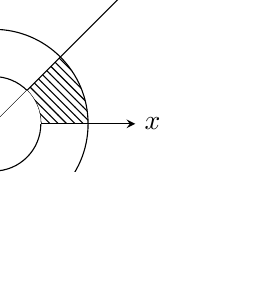
\begin{tikzpicture}[scale = 0.6]
			\def\xMIN{-1};
			\def\xMAX{3};
			\def\yMIN{-1};
			\def\yMAX{3};

			\def\PI{22/7};

			\begin{scope}[-stealth]
				\draw (\xMIN,0) -- (\xMAX,0) node [right] {$x$};
				\draw (0,\yMIN) -- (0,\yMAX) node [above] {$y$};
			\end{scope}

			\begin{scope}
				\clip (\xMIN,\yMIN) rectangle (\xMAX,\yMAX);
				\draw (\xMIN,\yMIN) -- (\xMAX,\xMAX);
				\draw (0,0) circle (1);
				\draw (0,0) circle (2);
			\end{scope}

			\begin{scope}
				\clip (0,0) -- (\xMAX,\yMAX) -- (\xMAX,0) -- cycle;
				\fill [pattern = north west lines] (0,0) circle (2);
				\fill [white] (0,0) circle (1);
			\end{scope}
		\end{tikzpicture}
	\end{figure}
	Therefore, it can be written as $S = \left\{ (r,\theta) | 1 \le r \le 2 , 0 \le \theta \le \frac{\pi}{4} \right\}$.\\
	Therefore,
	\begin{align*}
		\iint\limits_{R} x y \dif x \dif y & = \int\limits_{0}^{\frac{\pi}{4}} \int\limits_{1}^{2} r \cos \theta r \sin \theta r \dif r \dif \theta     \\
                                                   & = \int\limits_{1}^{2} r^3 \dif r \cdot \int\limits_{0}^{\frac{\pi}{4}} \cos \theta \sin \theta \dif \theta \\
                                                   & = \frac{15}{4} \cdot \frac{1}{4}                                                                           \\
                                                   & = \frac{15}{16}
	\end{align*}
\end{solution}

\begin{theorem}
	Let $D$ be a domain, written as $D_{\mathrm{I}}$ in polar coordinates, i.e.,
	\begin{equation*}
		D_{\mathrm{I}} = \left\{ (r,\theta) | a \le r \le b , g_1(r) \le \theta \le g_2(r) \right\}
	\end{equation*}
	and let $f(x,y)$ be continuous on $D_{\mathrm{I}}$.\\
	Then,
	\begin{equation*}
		\iint\limits_{D_{\mathrm{I}}} f(x,y) \dif x \dif y = \int\limits_{a}^{b} \int\limits_{g_1(r)}^{g_2(r)} f(r \cos \theta, r \sin \theta) r \dif \theta \dif r
	\end{equation*}
\end{theorem}

\begin{theorem}
	Let $D$ be a domain, written as $D_{\mathrm{II}}$ in polar coordinates, i.e.,
	\begin{equation*}
		D_{\mathrm{I}} = \left\{ (r,\theta) | \alpha \le \theta \le \beta , h_1(\theta) \le r \le h_2(\theta) \right\}
	\end{equation*}
	and let $f(x,y)$ be continuous on $D_{\mathrm{II}}$.\\
	Then,
	\begin{equation*}
		\iint\limits_{D_{\mathrm{II}}} f(x,y) \dif x \dif y = \int\limits_{\alpha}^{\beta} \int\limits_{h_1(\theta)}^{h_2(\theta)} f(r \cos \theta, r \sin \theta) r \dif r\dif \theta
	\end{equation*}
\end{theorem}

\section{Change of Variables in Triple Integrals}

\begin{definition}[Jacobian]
	Let
	\begin{align*}
		T(u,v,w) & = (x,y,z)
	\end{align*}
	be an operator.\\
	The determinant
	\begin{equation*}
		J = \frac{\partial(x,y,z)}{\partial(u,v,w)} =
			\begin{vmatrix}
				x_u & x_v & x_w \\
				y_u & y_v & y_w \\
				z_u & z_v & z_w \\
			\end{vmatrix}
	\end{equation*}
	is called the Jacobian of the operator $T$.
\end{definition}

\begin{theorem}
	Let $R$ and $S$ be domains of the first, second, or third kind.\\
	Let the operator $T$ from $S$ to $R$ be one-to-one and onto.\\
	Therefore, the inverse operator $T^{-1}$ exists.\\
	Also, let $T$ be a $C^1$ operator, i.e. $\exists x_u$, $\exists x_v$, $\exists x_w$, $\exists y_u$, $\exists y_v$, $\exists y_w$, $\exists z_u$, $\exists z_v$, $\exists z_w$, which are continuous on $S$.\\
	Let $f(x,y,z)$ be a continuous function on $R$.\\
	Then,
	\begin{equation*}
		\iint\limits_{R} f(x,y,z) \dif x \dif y \dif z = \iint\limits_{S} f\left( x(u,v,w), y(u,v,w), z(u,v,w) \right) |J| \dif u \dif v \dif w
	\end{equation*}
\end{theorem}

\subsection{Cylindrical Coordinates}

Cylindrical coordinates are a special case of change of variables.\\
The operator for the change of variables is
\begin{align*}
	T(r,\theta,z) & = (x,y,z)
\end{align*}
where
\begin{align*}
	x & = r \cos \theta \\
	y & = r \sin \theta \\
	z & = z
\end{align*}
Therefore,
\begin{align*}
	J &=
		\begin{vmatrix}
			x_r & x_{\theta} & x_z \\
			y_r & y_{\theta} & y_z \\
			z_r & z_{\theta} & z_z \\
		\end{vmatrix}\\
	  &=
		\begin{vmatrix}
			\cos \theta & -r \sin \theta & 0 \\
			\sin \theta & r \cos \theta  & 0 \\
			0           & 0              & 1 \\
		\end{vmatrix}\\
	  &= r \cos^2 \theta + r \sin^2 \theta\\
	  &= r
\end{align*}

\begin{question}
	Calculate the iterative integral
	\begin{align*}
		I & = \int\limits_{-2}^{2} \int\limits_{-\sqrt{4 - x^2}}^{\sqrt{4 - x^2}} \int\limits_{\sqrt{x^2 + y^2}}^{2} \left( x^2 + y^2 \right) \dif z \dif y \dif x
	\end{align*}
\end{question}

\begin{solution}
	The domain $\left\{ (x,y) | -2 \le x \le 2 , -\sqrt{4 - x^2} \le y \le \sqrt{4 - x^2} \right\}$ is a circle of radius $2$.\\
	As $\sqrt{x^2 + y^2} \le z \le 2$, the domain $E$, where $-2 \le x \le 2$, $-\sqrt{4 - x^2} \le y \le \sqrt{4 - x^2}$, $\sqrt{x^2 + y^2} \le z \le 2$ is a cone, with the circular cross section of radius $x^2 + y^2$.\\
	Therefore,
	\begin{align*}
		I & = \int\limits_{-2}^{2} \int\limits_{-\sqrt{4 - x^2}}^{\sqrt{4 - x^2}} \int\limits_{\sqrt{x^2 + y^2}}^{2} \left( x^2 + y^2 \right) \dif z \dif y \dif x \\
                  & = \iiint\limits_{E} \left( x^2 + y^2 \right) \dif x \dif y \dif z
	\end{align*}
	Therefore, let $D_{\mathrm{I}} = \left\{ (r,\theta,z) | 0 \le r \le 2 , 0 \le \theta \le 2 \pi , r \le z \le 2 \right\}$.\\
	Therefore,
	\begin{align*}
		I & = \int\limits_{-2}^{2} \int\limits_{-\sqrt{4 - x^2}}^{\sqrt{4 - x^2}} \int\limits_{\sqrt{x^2 + y^2}}^{2} \left( x^2 + y^2 \right) \dif z \dif y \dif x \\
                  & = \iiint\limits_{E} \left( x^2 + y^2 \right) \dif x \dif y \dif z                                                                                      \\
                  & = \iiint\limits_{D_{\mathrm{I}}} r^2 \cdot r \dif r \dif \theta \dif z                                                                                 \\
                  & = \int\limits_{0}^{2 \pi} \int\limits_{0}^{2} \int\limits_{r}^{2} r^3 \dif z \dif r \dif \theta                                                        \\
                  & = \int\limits_{0}^{2 \pi} \int\limits_{0}^{2} \left. r^3 z \right|_{z = r}^{z = 2} \dif r \dif \theta                                                  \\
                  & = \int\limits_{0}^{2 \pi} \int\limits_{0}^{2} \left( 2 r^3 - r^4 \right) \dif r \dif \theta                                                            \\
                  & = \frac{16 \pi}{5}
	\end{align*}
\end{solution}

\subsection{Spherical Coordinates}

Spherical coordinates are a special case of change of variables.\\
The operator for the change of variables is
\begin{align*}
	T(\rho,\theta,\varphi) & = (x,y,z)
\end{align*}
where
\begin{align*}
	x & = \rho \cos \theta \sin \varphi \\
	y & = \rho \sin \theta \sin \varphi \\
	z & = \rho \cos \varphi
\end{align*}
Therefore,
\begin{align*}
	J &=
		\begin{vmatrix}
			x_{\rho} & x_{\theta} & x_{\varphi} \\
			y_{\rho} & y_{\theta} & y_{\varphi} \\
			z_{\rho} & z_{\theta} & z_{\varphi} \\
		\end{vmatrix}\\
	  &=
		\begin{vmatrix}
			\cos \theta \sin \theta & -r \sin \theta \sin \varphi & r \cos \theta \cos \varphi \\
			\sin \theta \sin \theta & r \cos \theta \sin \varphi  & r \sin \theta \cos \varphi \\
			\cos \varphi            & 0                           & -r \sin \varphi            \\
		\end{vmatrix}\\
	  &= -\rho^2 \sin \varphi
\end{align*}

\begin{question}
	Given the sphere $B : x^2 + y^2 + z^2 \le 1$, find $I = \iiint\limits_{B} e^{\left( x^2 + y^2 + z^2 \right)^{\frac{3}{2}}} \dif x \dif y \dif z$.
\end{question}

\begin{solution}
	\begin{align*}
		I & = \iiint\limits_{B} e^{\left( x^2 + y^2 + z^2 \right)^{\frac{3}{2}}} \dif x \dif y \dif z                                                         \\
                  & = \int\limits_{0}^{\pi} \int\limits_{0}^{2 \pi} \int\limits_{0}^{1} e^{\rho^{\frac{3}{2}}} |J| \dif \rho \dif \theta \dif \varphi                 \\
                  & = \int\limits_{0}^{\pi} \int\limits_{0}^{2 \pi} \int\limits_{0}^{1} e^{\rho^{\frac{3}{2}}} \rho^2 \sin \varphi \dif \rho \dif \theta \dif \varphi \\
                  & = \int\limits_{0}^{\pi} \int\limits_{0}^{2 \pi} \left. \frac{e^{\rho^3}}{3} \sin \varphi \right|_{\rho = 0}^{\rho = 1} \dif \theta \dif \varphi   \\
                  & = \frac{e - 1}{3} \int\limits_{0}^{\pi} \int\limits_{0}^{2 \pi} \sin \varphi \dif \theta \dif \varphi                                             \\
                  & = \frac{e - 1}{3} \int\limits_{0}^{\pi} \sin \varphi \cdot 2 \pi \dif \varphi                                                                     \\
                  & = 2 \pi \frac{e - 1}{3} \left. (- \cos \theta) \right|_{0}^{\pi}                                                                                  \\
                  & = \frac{4 \pi (e - 1)}{3}
	\end{align*}
\end{solution}

\begin{question}
	Calculate the volume of a body which is situated above the cone $z = \sqrt{x^2 + y^2}$ and under the sphere $x^2 + y^2 + z^2 = z$.
\end{question}

\begin{solution}
	\begin{align*}
		x^2 + y^2 + z^2                                         & = z \\
		\therefore x^2 + y^2 + z^2 - z                          & = 0 \\
		\therefore x^2 + y^2 + \left( z - \frac{1}{2} \right)^2 & = \frac{1}{4}
	\end{align*}
	Therefore, the sphere has centre $\left( 0 , 0 , \frac{1}{2} \right)$ and radius $\frac{1}{2}$.\\
	Therefore, the cone and the sphere intersect each other at $z = \frac{1}{2}$.
	The intersection is a circle with radius $\frac{1}{2}$.\\
	Therefore, the body is made of a cone of base radius $\frac{1}{2}$ and height $\frac{1}{2}$, and a hemisphere of radius $\frac{1}{2}$.\\
	In Cartesian coordinates, the sphere is $x^2 + y^2 + z^2 = z$.\\
	Therefore, in spherical coordinates, the sphere is $\rho^2 = \rho \cos \varphi$.
	Therefore,
	\begin{align*}
		V & = \iiint \dif x \dif y \dif z                                                                                                                                              \\
                  & = \int\limits_{0}^{2 \pi} \int\limits_{0}^{\frac{\pi}{4}} \int\limits_{0}^{\cos \varphi} \rho^2 \sin \varphi \dif \rho \dif \varphi \dif \theta                            \\
                  & = \int\limits_{0}^{2 \pi} \int\limits_{0}^{\frac{\pi}{4}} \left. \frac{\rho^3}{3} \sin \varphi \right|_{\rho = 0}^{\rho = \cos \varphi} \dif \rho \dif \varphi \dif \theta \\
                  & = \int\limits_{0}^{2 \pi} \int\limits_{0}^{\frac{\pi}{4}} \frac{1}{3} \cos^3 \varphi \sin \varphi \dif \varphi \dif \theta                                                 \\
                  & = 2 \pi \cdot \left. \left( -\frac{\cos^4 \pi}{12} \right) \right|_{0}^{\frac{\pi}{4}}                                                                                     \\
                  & = 2 \pi \left( -\frac{1}{48} + \frac{1}{12} \right)                                                                                                                        \\
                  & = 2 \pi \left( \frac{3}{48} \right)                                                                                                                                        \\
                  & = \frac{\pi}{8}
	\end{align*}
\end{solution}

\section{Line Integrals of Scalar Functions}

\begin{definition}[Smooth curve]
	A curve $C$ which is parametrically given as $\overline{r}(t) = \left( x(t) , y(t) , z(t) \right)$, $t : a \to b$ is said to be smooth if $\overline{r}(t)$ is a continuous function on $[a,b]$, $\overline{r}'(t) \neq 0$ on $(a,b)$, and $\overline{r}'(t)$is continuous on $(a,b)$.
\end{definition}

\begin{theorem}
	If $f(x,y,z)$ is continuous and $C$ is smooth, then
	\begin{align*}
		\int\limits_{C} f(x,y,z) \dif s & = \int\limits_{a}^{b} f\left( x(t) , y(t), z(t) \right) \sqrt{\left( x'(t) \right)^2 + \left( y'(t) \right)^2 + \left( z'(t) \right)^2} \dif t
	\end{align*}
\end{theorem}

\begin{theorem}
	If $f(x,y,z)$ is continuous and $C$ is smooth, then
	\begin{align*}
		\int\limits_{C} f(x,y,z) \dif x & = \int\limits_{a}^{b} f\left( x(t) , y(t) , z(t) \right) x'(t) \dif t
	\end{align*}
	\begin{align*}
		\int\limits_{C} f(x,y,z) \dif y & = \int\limits_{a}^{b} f\left( x(t) , y(t) , z(t) \right) y'(t) \dif t
	\end{align*}
	\begin{align*}
		\int\limits_{C} f(x,y,z) \dif z & = \int\limits_{a}^{b} f\left( x(t) , y(t) , z(t) \right) z'(t) \dif t
	\end{align*}
\end{theorem}

\begin{question}
	Calculate $\int\limits_{C} y \dif x + z \dif y + x \dif z$ for $C$ as shown.
	\begin{figure}[H]
		\begin{tikzpicture}[scale = 0.5]
			\def\xMIN{-1};
			\def\xMAX{6};
			\def\yMIN{-1};
			\def\yMAX{6};
			\def\zMIN{-1};
			\def\zMAX{6};

			\def\PI{22/7};

			\begin{scope}[-stealth]
				\draw (\xMIN,0,0) -- (\xMAX,0,0) node [right] {$x$};
				\draw (0,\yMIN,0) -- (0,\yMAX,0) node [above] {$y$};
				\draw (0,0,\zMIN) -- (0,0,\zMAX) node [above] {$z$};
			\end{scope}

			\begin{scope}
				\node [below] at (2,0,0) {$(2,0,0)$};
				\node [left] at (3,4,5) {$(3,4,5)$};
				\node [above] at (3,4,0) {$(3,4,0)$};
			\end{scope}

			\begin{scope}[-stealth]
				\draw (2,0,0) -- (3,4,5);
				\draw (3,4,5) -- (3,4,0);
			\end{scope}
		\end{tikzpicture}
	\end{figure}
\end{question}

\begin{solution}
	\begin{align*}
		C &= C_1 \cup C_2
	\end{align*}
	Therefore, for $t : 0 \to 1$,
	\begin{gather*}
		C_1 : \overline{r}(t) = (2 + 1 \cdot t , 0 + 4 \cdot t , 0 + 5 \cdot t) \\
		C_2 : \overline{r}(t) = (3 + 0 \cdot t , 4 + 0 \cdot t , 5 - 5 \cdot t)
	\end{gather*}
	Therefore,
	\begin{align*}
		\int\limits_{C} y \dif x + z \dif y + x \dif z & = \int\limits_{C_1} y \dif x + z \dif y + x \dif z + \int\limits_{C_2} y \dif x + z \dif y + x \dif z    \\
                                                               & = \quad \int\limits_{0}^{1} \left( y_1(t) {x_1}'(t) + z_1(t) {y_1}'(t) + x_1(t) {z_1}'(t) \right) \dif t \\
                                                               & \quad + \int\limits_{0}^{1} \left( y_2(t) {x_2}'(t) + z_2(t) {y_2}'(t) + x_2(t) {z_2}'(t) \right) \dif t \\
                                                               & = \quad \int\limits_{0}^{1} \left( 4 t + 5 t \cdot 4 + (2 + t) \cdot 5 \right) \dif t                    \\
                                                               & + \quad \int\limits_{0}^{1} \left( 4 \cdot 0 + (5 - 5 t) \cdot 0 + 3 \cdot (-5) \right) \dif t           \\
                                                               & = \int\limits_{0}^{1} (29 t - 5) \dif t                                                                  \\
                                                               & = \left. \left( 29 \frac{t^2}{2} - 5 t \right) \right|_{0}^{1}                                           \\
                                                               & = \frac{19}{2}
	\end{align*}
\end{solution}

\section{Line Integrals of Vector Functions}

\begin{theorem}
	If $C : \overline{r}(t) = \left( x(t) , y(t) , z(t) \right)$, $t : a \to b$, then
	\begin{align*}
		W & =\int\limits_{C} \overline{F} \cdot \hat{T} \dif s                                                                                                                \\
                  & = \int\limits_{a}^{b} \left( \overline{F}\left( \overline{r}(t) \right) \right) \cdot {\overline{r}}'(t) \dif t                                                           \\
                  & = \int\limits_{C} \overline{F} \cdot \dif \overline{r}                                                                                                            \\
                  & = \int\limits_{a}^{b} \left( P\left( \overline{r}(t) \right) x'(t) + Q\left( \overline{r}(t) \right) y'(t) + R\left( \overline{r}(t) \right) z'(t) \right) \dif t \\
                  & = \int\limits_{C} P \dif x + Q \dif y + R \dif z
	\end{align*}
\end{theorem}

\begin{theorem}[Fundamental Theorem of Line Integrals]
	Let $C$ be a smooth curve in $\mathbb{R}^2$ or $\mathbb{R}^3$ given parametrically by $\overline{r}(t)$, $t : a \to b$.
	Let $f$ be a continuous function of $(x,y)$ or $(x,y,z)$, on $C$, and $\nabla f$ be a continuous vector function in a connected domain $D$ which contains $C$.
	Then
	\begin{align*}
		W & = \int\limits_{C} \nabla f \cdot \hat{T} \dif s                     \\
                  & = f\left( \overline{r}(b) \right) - f\left( \overline{r}(a) \right) \\
                  & = f(B) - f(A)
	\end{align*}
	\label{Fundamental_Theorem_of_Line_Integrals}
\end{theorem}

\begin{definition}[Simple curve]
	A curve $C$ is called a simple curve if it does not intersect itself.
\end{definition}

\begin{definition}[Connected domain]
	A domain $D \subset \mathbb{R}^2$ is called connected if for any two points from $D$, the is a path $C$ which connects the points and remains in $D$.
\end{definition}

\begin{definition}[Simple connected domain]
	A connected domain $D \subset \mathbb{R}^2$ is called simple connected if any simple closed curve from $D$ contains inside itself only points in $D$.
\end{definition}

\begin{definition}[Curve with positive orientation]
	A simple closed curve $C$ is called a curve with a positive orientation, or with anti-clockwise orientation if the domain $D$ bounded by $C$ always remains on the left when we circulate over $C$ by $\overline{r}(t), t : a \to b$.
\end{definition}

\section{Surface Integrals of Scalar Functions}

\begin{definition}[Parametic representation of surfaces]
	Let the surface $S$ be given by
	\begin{align*}
		\overline{r}(u,v) & = \left( f(u,v) , g(u,v) , h(u,v) \right)
	\end{align*}
	The equations
	\begin{align*}
		x & = f(u,v) \\
		y & = g(u,v) \\
		z & = h(u,v)
	\end{align*}
	are called the parametric equations of $S$
\end{definition}

\begin{definition}
	If a smooth surface $S$ is given by $\overline{r}(u,v) = \left( x(u,v) , y(u,v) , z(u,v) \right)$, $u,v \in D$ and $\overline{r}(u,v)$ is one-to-one, then the surface area of $S$ is
	\begin{align*}
		A & = \iint\limits_{D} \left| \overline{r}_u \times \overline{r}_v \right| \dif u \dif v
	\end{align*}
	where
	\begin{align*}
		\overline{r}_u & = (x_u, y_u, z_u) \\
		\overline{r}_v & = (x_v, y_v, z_v)
	\end{align*}
\end{definition}

\begin{theorem}
	If $S$ is smooth and given by $z = g(x,y)$, $(x,y) \in D$, then
	\begin{align*}
		\iint\limits_{S} f(x,y,z) \dif S &= \iint\limits_{D} f\left( x , y , g(x,y) \right) \sqrt{1 + (g_x)^2 + (g_y)^2} \dif x \dif y
	\end{align*}
\end{theorem}
\begin{theorem}
	If $S$ is smooth and given parametrically by $\overline{r}(u,v) = \left( x(u,v) , y(u,v) , z(u,v) \right)$, $(u,v) \in D$, then
	\begin{align*}
		\iint\limits_{S} f(x,y,z) \dif S &= \iint\limits_{D} f\left( \overline{r}(u,v) \right) \left| \overline{r}_u \times \overline{r}_v \right| \dif u \dif v
	\end{align*}
\end{theorem}

\begin{question}
	Find $\iint\limits_{S} x^2 \dif S$ where $S : x^2 + y^2 + z^2 = 1$.
\end{question}

\begin{solution}
	In spherical coordinates with $\rho = 1$,
	\begin{align*}
		x &= \cos \theta \sin \varphi\\
		y &= \sin \theta \sin \varphi\\
		z &= \cos \varphi
	\end{align*}
	Therefore,
	\begin{align*}
		\overline{r}(\theta , \varphi) & = (\sin \varphi \cos \theta , \sin \varphi \sin \theta , \cos \varphi)
	\end{align*}
	Therefore,
	\begin{align*}
		\overline{r}_{\theta}  & = (-\sin \varphi \sin \theta , \sin \varphi \cos \theta , 0) \\
		\overline{r}_{\varphi} & = (\cos \varphi \cos \theta , \cos \varphi \sin \theta , -\sin \varphi)
	\end{align*}
	Therefore,
	\begin{align*}
		\overline{r}_{\theta} \times \overline{r}_{\varphi} &=
			\begin{vmatrix}
				\hat{i}                   & \hat{j}                  & \hat{k}       \\
				-\sin \varphi \sin \theta & \sin \varphi \cos \theta & 0             \\
				\cos \varphi \cos \theta  & \cos \varphi \sin \theta & -\sin \varphi \\
			\end{vmatrix}\\
		&= \quad \hat{i} \left( -\sin^2 \varphi \cos \theta \right)\\
		&\quad - \hat{j} \left( \sin^2 \varphi \sin \theta \right)\\
		&\quad + \hat{k} \left( -\sin \varphi \cos \varphi \sin^2 \theta - \sin \varphi \cos \varphi \cos^2 \theta \right)
	\end{align*}
	Therefore,
	\begin{align*}
		\left| \overline{r}_{\theta} \times \overline{r}_{\varphi} \right| & = \sqrt{\sin^4 \varphi \cos^2 \theta + \sin^4 \varphi \sin^2 \theta + \sin^2 \varphi \cos^2 \varphi} \\
                                                                                   & = \sqrt{\sin^4 \varphi + \sin^2 \varphi \cos^2 \varphi}                                              \\
                                                                                   & = \sqrt{\sin^2 \varphi}                                                                              \\
                                                                                   & = \sin \varphi
	\end{align*}
	Therefore,
	\begin{align*}
		\iint\limits_{S} x^2 \dif S & = \iint\limits_{D} (\cos \theta \sin \varphi)^2 \sin \varphi \dif \theta \dif \varphi                                                                                             \\
                                            & = \int\limits_{0}^{2 \pi} \int\limits_{0}^{\pi} \sin^3 \varphi \cos^2 \theta \dif \varphi \dif \theta                                                                             \\
                                            & = \int\limits_{0}^{\pi} \sin^3 \varphi \dif \varphi \int\limits_{0}^{2 \pi} \cos^2 \theta \dif \theta                                                                             \\
                                            & = \int\limits_{0}^{\pi} \left( 1 - \cos^2 \varphi \right) \sin \varphi \dif \varphi \int\limits_{0}^{2 \pi} \frac{1 + \cos 2 \theta}{2} \dif \theta                               \\
                                            & = \int\limits_{0}^{\pi} \left( \sin \varphi - \cos^2 \varphi \sin \varphi \right) \dif \varphi \left( \left. \frac{\theta}{2} + \frac{\sin 2 \theta}{4} \right|_{0}^{\pi} \right) \\
                                            & = \frac{4 \pi}{3}
	\end{align*}
\end{solution}

\section{Surface Integrals of Vector Functions}

\begin{definition}[Oriented surface]
	If a normal vector $\overline{n}(x,y,z)$ to the surface $S$ is continuously changing on $S$ then $S$ is said to be an oriented surface.
\end{definition}

\begin{theorem}
	If a surface is given by $F(x,y,z) = k$, then $\nabla F$ is a normal vector to the surface at a point on it.
\end{theorem}

\begin{definition}[Surface with positive orientation]
	A surface $S$ is said to have positive orientation if $\hat{n}$ is positive.\\
	A closed surface $S$ is said to have positive orientation if $\hat{n}$ is directed outwards.
\end{definition}

\begin{definition}[Surface Integral of Vector Functions]
	If 
	\begin{align*}
		\overline{F}(x,y,z) = \left( P(x,y,z) , Q(x,y,z) , R(x,y,z) \right)
	\end{align*}
	is a continuous vector function on $S$ with orientation $\hat{n}$, then the surface integral of $\overline{F}$ over $\overline{S}$ is
	\begin{align*}
		\iint\limits_{S} \overline{F} \cdot \dif \overline{S} & = \iint\limits_{S} \overline{F} \cdot \hat{n} \dif S
	\end{align*}
	This integral is also called the flux of $\overline{F}$ through $\overline{S}$ in direction $\hat{n}$.
\end{definition}

\begin{theorem}
	Let
	\begin{align*}
		\overline{F}(x,y,z) = \left( P(x,y,z) , Q(x,y,z) , R(x,y,z) \right)
	\end{align*}
	~\\
	If $S : z = g(x,y)$, $(x,y) \in D$, then,
	\begin{align*}
		\iint\limits_{S} \overline{F} \cdot \dif \overline{S} & = \iint\limits_{S} \overline{F} \cdot \hat{n} \dif S \\
                                                                      & = \iint\limits_{D} \left( -P g_x - Q g_y + R \right) \dif x \dif y
	\end{align*}
	for $S$ with positive orientation, and
	\begin{align*}
		\iint\limits_{S} \overline{F} \cdot \dif \overline{S} & = \iint\limits_{S} \overline{F} \cdot \hat{n} \dif S \\
                                                                      & = -\iint\limits_{D} \left( -P g_x - Q g_y + R \right) \dif x \dif y
	\end{align*}
	for $S$ with negative orientation.
	~\\
	If $S$ is given parametrically as
	\begin{align*}
		\overline{r}(u,v) & = \left( x(u,v) , y(u,v) , z(u,v) \right)
	\end{align*}
	for $(u,v) \in D$, then
	\begin{align*}
		\iint\limits_{S} \overline{F} \cdot \dif \overline{S} & = \iint\limits_{S} \overline{F} \cdot \hat{n} \dif S \\
                                                                      & = \iint\limits_{D} \overline{F} \cdot \left( \overline{r}_u \times \overline{r}_v \right) \dif u \dif v
	\end{align*}
	~\\
	If $S$ is closed and given parametrically, it can be solved as above.\\
	If $S$ is closed and not given parametrically, it can be divided into surfaces of the first kind, and each of the integrals over the smaller surfaces can be solved as above.
\end{theorem}

\begin{question}
	Given
	\begin{align*}
		\overline{F} & = (x,y,z)
	\end{align*}
	Calculate $\iint\limits_{S} \overline{F} \cdot \hat{n} \dif S$, where $S : x^2 + y^2 + z^2 = 1$.
\end{question}

\begin{solution}
	The surface $S$ is given by
	\begin{align*}
		x^2 + y^2 + z^2 & = 1 \\
		\therefore z    & = \pm \sqrt{1 - x^2 - y^2}
	\end{align*}
	Therefore, let
	\begin{align*}
		S_1 & = -\sqrt{1 - x^2 - y^2} \\
		S_2 & = \sqrt{1 - x^2 - y^2}
	\end{align*}
	Therefore,
	\begin{align*}
		\iint\limits_{S} \overline{F} \cdot \hat{n} \dif S & = \iint\limits_{S_1} \overline{F} \cdot \hat{n} \dif S + \iint\limits_{S_2} \overline{F} \cdot \hat{n} \dif S                         \\
                                                                   & = -\iint\limits_{D} \left( -P (g_1)_x - Q (g_1)_y + R \right) \dif x \dif y                                                           \\
                                                                   & \quad + \iint\limits_{D} \left( -P (g_1)_x - Q (g_1)_y + R \right) \dif x \dif y                                                      \\
                                                                   & = 2 \iint\limits_{D} \left( \frac{x^2}{\sqrt{1 - x^2 - y^2}} + \frac{y^2}{\sqrt{1 - x^2 - y^2}} + \sqrt{1 - x^2 - y^2} \right) \dif A \\
                                                                   & = 2 \iint\limits_{D} \frac{1}{\sqrt{1 - x^2 - y^2}} \dif x \dif y                                                                     \\
                                                                   & = 2 \int\limits_{0}^{1} \int\limits_{0}^{2 \pi} \frac{1}{1 - r^2} r \dif \theta \dif r                                                \\
                                                                   & = 4 \pi
	\end{align*}
\end{solution}

\begin{question}
	Given
	\begin{align*}
		\overline{F} & = (x,y,z)
	\end{align*}
	Calculate $\iint\limits_{S} \overline{F} \cdot \hat{n} \dif S$, where $S : x^2 + y^2 + z^2 = 1$, using parametric representation.
\end{question}

\begin{solution}
	$S$ is given parametrically by
	\begin{align*}
		\overline{r}(\theta,\varphi) = \left( x(\theta,\varphi) , y(\theta,\varphi) , z(\theta,\varphi) \right)
	\end{align*}
	where
	\begin{align*}
		x(\theta,\varphi) & = \cos \theta \sin \varphi \\
		y(\theta,\varphi) & = \sin \theta \sin \varphi \\
		z(\theta,\varphi) & = \cos \varphi
	\end{align*}
	with $D : \{0 \le \theta \le 2 \pi , 0 \le \varphi \le \pi\}$.\\
	Therefore,
	\begin{align*}
		\overline{r}_{\theta} \times \overline{r}_{\varphi} & = \left( -\cos \theta \sin^2 \varphi , -\sin \theta \sin^2 \varphi , -\sin \varphi \cos \varphi \right)
	\end{align*}
	If $\theta = \frac{\pi}{2}$, $\varphi = \frac{\pi}{2}$,
	\begin{align*}
		\overline{r}_{\theta} \times \overline{r}_{\varphi} & = (0,-1,0)
	\end{align*}
	However, the positive normal to $S$ at that point is positively directed.\\
	Therefore,
	\begin{align*}
		\iint\limits_{S} \overline{F} \cdot \hat{n} \dif S & = -\iint\limits_{D} \overline{F} \cdot \left( \overline{r}_{\theta} \times \overline{r}_{\varphi} \right) \dif \theta \dif \varphi                     \\
                                                                   & = -\iint\limits_{D} \left( -\cos^2 \theta \sin^3 \varphi - \sin^2 \theta \sin^3 \varphi - \cos^2 \varphi \sin \varphi \right) \dif \theta \dif \varphi \\
                                                                   & = \iint\limits_{D} \left( \sin^3 \varphi + \cos^2 \varphi \sin \varphi \right) \dif \theta \dif \varphi                                                \\
                                                                   & = \iint\limits_{D} \sin \varphi \dif \theta \dif \varphi                                                                                               \\
                                                                   & = \int\limits_{0}^{2 \pi} \int\limits_{0}^{\pi} \sin \varphi \dif \varphi \dif \theta                                                                  \\
                                                                   & = \int\limits_{0}^{2 \pi} \dif \theta \int\limits_{0}^{\pi} \sin \varphi \dif \varphi                                                                  \\
                                                                   & = 2 \pi \left. \left( -\cos \varphi \right) \right|_{0}^{\pi}                                                                                          \\
                                                                   & = 4 \pi
	\end{align*}
\end{solution}

\section{Green's Theorem}

\begin{definition}[Curl/Rotor]
	If
	\begin{align*}
		\overline{F}(x,y,z) & = \left( P(x,y,z) , Q(x,y,z) , R(x,y,z) \right)
	\end{align*}
	then
	\begin{align*}
		\curl \overline{R} &= \nabla \times \overline{F}\\
		                &=
			\begin{vmatrix}
				\hat{i}   & \hat{j}   & \hat{k}   \\
				\dpd{}{x} & \dpd{}{y} & \dpd{}{z} \\
				P         & Q         & R
			\end{vmatrix}
	\end{align*}
\end{definition}

\begin{definition}[Divergence]
	If
	\begin{align*}
		\overline{F}(x,y,z) & = \left( P(x,y,z) , Q(x,y,z) , R(x,y,z) \right)
	\end{align*}
	then
	\begin{equation*}
		\divergence \overline{R} = \nabla \cdot \overline{F} = \dpd{P}{x} + \dpd{Q}{y} + \dpd{R}{z}
	\end{equation*}
\end{definition}

\begin{theorem}
	If a vector field $\overline{F}(x,y,z)$ is defined on $\mathbb{R}^3$, if there exist continuous first order partial derivatives of $P$, $Q$, $R$, and if $\curl \overline{F} = 0$, then $\overline{F}$ is a conservative vector field.\\
	In this case, $\exists f(x,y,z)$, such that $\overline{F} = \nabla f$.
\end{theorem}

\begin{theorem}[Green's Theorem]
	Let $C$ be a piecewise smooth, simple, and closed curve in $\mathbb{R}^2$ with positive orientation.
	Let $D$ be a domain bounded by $C$.
	If there exist continuous first order partial derivatives of $P(x,y)$ and $Q(x,y)$ in an open domain which contains $D$, then
	\begin{align*}
		W & = \int\limits_{C} \overline{F} \cdot \hat{T} \dif s = \int\limits_{C} P \dif x + Q \dif y\\
                  & = \iint\limits_{D} (Q_x - P_y) \dif A = \iint\limits_{D} \curl \overline{F} \cdot \hat{k} \dif A = \iint\limits_{D} \divergence \overline{F} \dif A
	\end{align*}
	\label{Green's_Theorem}
\end{theorem}

\section{Stoke's Theorem}

\begin{definition}[Curve with positive orientation]
	Let $S$ be an oriented surface with normal $\hat{n}$ and let $C$ be a curve bounding $S$.
	$C$ is called a curve with positive orientation with respect to $S$ if, as we walk on $C$ in this direction and with our head in the direction of $\hat{n}$, the surface $S$ is always on our left.
\end{definition}

\begin{theorem}[Stoke's Theorem]
	Let $S$ be a piecewise smooth surface with normal $\hat{n}$ and let $S$ be bounded by a curve $C$ which is piecewise smooth, simple, closed and with positive orientation with respect to $S$.
	Let $\overline{F}(x,y,z) = \left( P(x,y,z), Q(x,y,z), R(x,y,z) \right)$ be a vector field such that there exist continuous first order partial derivatives of $P$, $Q$, $R$ in an open domain of $\mathbb{R}^3$ which contains $S$.
	Then 
	\begin{equation*}
		\int\limits_{C} \overline{F} \cdot \hat{T} \dif s = \iint\limits_{S} \curl \overline{F} \cdot \hat{n} \dif S
	\end{equation*}
	\nameref{Stoke's_Theorem} is a generalization of \nameref{Green's_Theorem}.
	\label{Stoke's_Theorem}
\end{theorem}

\section{Gauss' Theorem}

\begin{theorem}
	Let $E$ be a body bounded by a surface $S$, with a positive orientation of $S$.
	Let
	\begin{align*}
		\overline{F} & = (P,Q,R)
	\end{align*}
	be a vector field such that there exist continuous first order partial derivatives of $P$, $Q$, and $Q$, in some open domain which contains $E$.
	Then,
	\begin{align*}
		\iint\limits_{S} \overline{F} \cdot \hat{n} \dif S & = \iiint\limits_{E} \divergence \overline{F} \dif V
	\end{align*}
	\label{Gauss's_Theorem}
\end{theorem}

\begin{question}
	Find $\iint\limits_{S} \overline{F} \cdot \hat{n} \dif S$ where
	\begin{align*}
		\overline{F} & = \left( x y , y^2 + e^{x z^2} , \sin x y \right)
	\end{align*}
	and $S$ is a lateral surface of a body $E$ which is bounded by the parabolic cylinder $z = 1 - x^2$ and the planes $z = $, $y = 0$, and $y + z = 2$.
\end{question}

\begin{solution}
	\begin{align*}
		\iint\limits_{S} \overline{F} \cdot \hat{n} \dif S & = \iiint\limits_{E} \divergence \overline{F} \dif V                                          \\
                                                                   & = \iiint\limits_{E} (y + 2 y + 0) \dif V                                                     \\
                                                                   & = 3 \iiint\limits_{E_{\mathrm{II}}} y \dif V                                                 \\
                                                                   & = 3 \iint\limits_{D} \left( \int\limits_{0}^{2 - z} y \dif y \right) \dif A                  \\
                                                                   & = 3 \iint\limits_{D} \left. \frac{y^2}{2} \right|_{y = 0}^{y = 2 - z} \dif A                 \\
                                                                   & = \frac{3}{2} \iint\limits_{D} (2 - z)^2 \dif A                                              \\
                                                                   & = \frac{3}{2} \int\limits_{-1}^{1} \int\limits_{0}^{1 - x^2} (2 - z)^2 \dif z \dif x         \\
                                                                   & = \frac{184}{35}
	\end{align*}
\end{solution}

\begin{question}
	Verify \nameref{Stoke's_Theorem} when $\overline{F} = \left( -y^2 , x , z^2 \right)$ and $C$ is the intersecton like between the plane $y + z = 2$ and the culinder $x^2 + y^2 = 1$.
	The direction of $C$ is clockwise, when seen from above.
\end{question}

\begin{solution}
	Let $S$ be the circular surface enclosed by $C$.\\
	As $C$ is clockwise, when seen from above, $\hat{n}$ is negative.\\
	Let
	\begin{align*}
		x & = \cos t \\
		y & = \sin t
	\end{align*}
	Therefore, as $y + z = 2$,
	\begin{align*}
		z & = 2 - \sin t
	\end{align*}
	where, $t : 2 \pi \to 0$.\\
	$t$ goes from $2 \pi$ to $0$ and not from $0$ to $2 \pi$, as $C$ is directed clockwise, when seen from above.\\
	Therefore, the LHS is,
	\begin{align*}
		\int\limits_{C} \overline{F} \cdot \hat{T} \dif S & = \int\limits_{2 \pi}^{0} \left( P x'(t) + Q y'(t) + R z'(t) \right) \dif t                                                         \\
                                                                  & = \int\limits_{2 \pi}^{0} \left( -\sin^2 t \cdot -\sin t + \cos t \cdot \cos t + (2 - \sin t)^2 \cdot -\cos t \right) \dif t        \\
                                                                  & = \int\limits_{2 \pi}^{0} \left( \left( 1 - \cos^2 t \right) \sin t + \frac{1 + \cos 2 t}{2} - (2 - \sin t)^2 \cos t \right) \dif t \\
                                                                  & = \left. -\cos t + \frac{\cos^3 t}{3} + \frac{t}{2} + \frac{\sin 2 t}{4} + \frac{(2 - \sin t)^3}{3} \right|_{2 \pi}^{0}             \\
                                                                  & = -\pi
	\end{align*}
	~\\
	\begin{align*}
		\curl \overline{F} &= \nabla \times \overline{F}\\
		                   &=
			\begin{vmatrix}
				\hat{i}   & \hat{j}   & \hat{k}   \\
				\dpd{}{x} & \dpd{}{y} & \dpd{}{z} \\
				P         & Q         & R
			\end{vmatrix}\\
		                   &=
			\begin{vmatrix}
				\hat{i}   & \hat{j}   & \hat{k}   \\
				\dpd{}{x} & \dpd{}{y} & \dpd{}{z} \\
				-y^2      & x         & z^2
			\end{vmatrix}\\
		                   &= (0 - 0) \hat{i} - (0 - 0) \hat{j} + (1 + 2 y) \hat{k}\\
		                   &= (1 + 2 y) \hat{k}\\
		                   &= \tilde{P} \hat{i} + \tilde{Q} \hat{j} + \tilde{R} \hat{k}
	\end{align*}
	As $C$ is clockwise, when seen from above, $\hat{n}$ is negative.\\
	Therefore, the RHS is,
	\begin{align*}
		\iint\limits_{S} \curl \overline{F} \cdot \hat{n} \dif S & = -\iint\limits_{D} \left( -\tilde{P} g_x - \tilde{Q} q_y + \tilde{R} \right) \dif A                                               \\
                                                                         & = -\iint\limits_{D} \tilde{R} \dif A                                                                                               \\
                                                                         & = -\iint\limits_{D} (1 + 2 y) \dif A                                                                                               \\
                                                                         & = -\int\limits_{0}^{1} \int\limits_{0}^{2 \pi} (1 + 2 r \sin \theta) r \dif \theta \dif r                                          \\
                                                                         & = -\int\limits_{0}^{1} \int\limits_{0}^{2 \pi} r \dif \theta \dif r - \int\limits_{0}^{2 \pi} 2 r^2 \sin \theta \dif \theta \dif r \\
                                                                         & = -\int\limits_{0}^{1} r \dif r \int\limits_{0}^{2 \pi} \dif \theta                                                                \\
                                                                         & = -\pi
	\end{align*}
	\qed
\end{solution}

\end{multicols}

\end{spacing}

%\fontsize{12pt}{14.4pt}\selectfont

\begin{tabular}{|c|c|c|c|c|c|}
	\hline
	Surface & Equation & \multicolumn{3}{|c|}{Trace} & Graph\\
	\cline{3-5}
	& & $z = 0$ & $y = 0$ & $x = 0$ & \\
	\hline
	Hyperboloid of One Sheet  & $\frac{x^2}{a^2} + \frac{y^2}{b^2} - \frac{z^2}{c^2} = 1$  & ellipse              & hyperbola            & hyperbola             & 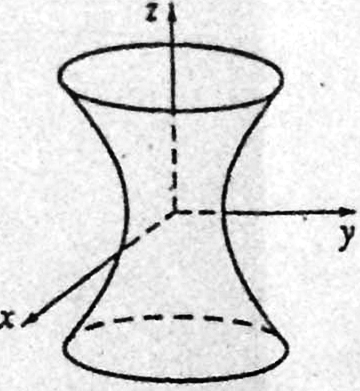
\includegraphics[height = 2cm]{Hyperboloid_of_1_sheet.jpg}  \\
	Hyperboloid of Two Sheets & $-\frac{x^2}{a^2} - \frac{y^2}{b^2} + \frac{z^2}{c^2} = 1$ & none                 & hyperbola            & hyperbola             & 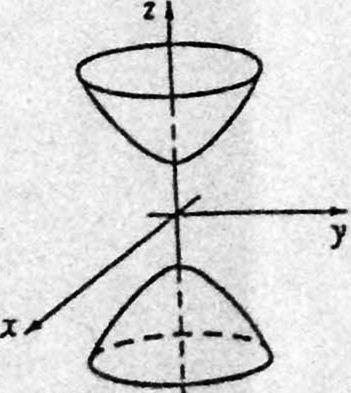
\includegraphics[height = 2cm]{Hyperboloid_of_2_sheets.jpg} \\
	Elliptic Cone             & $z^2 = \frac{x^2}{a^2} + \frac{y^2}{b^2}$                  & $(0,0,0)$            & 2 intersecting lines & 2 intersecting lines  & 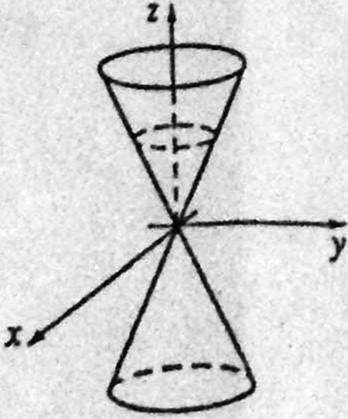
\includegraphics[height = 2cm]{Elliptic_cone.jpg}           \\
	Elliptic Paraboloid       & $z = \frac{x^2}{a^2} + \frac{y^2}{b^2}$                    & $(0,0,0)$            & upwards parabola     & upwards parabola      & 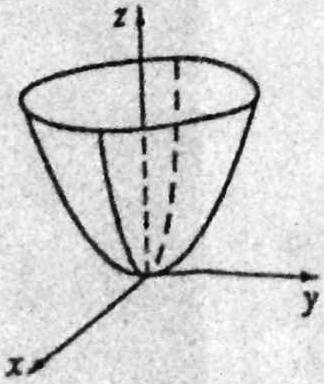
\includegraphics[height = 2cm]{Elliptic_paraboloid.jpg}     \\
	Hyperboloid Paraboloid    & $z = \frac{x^2}{a^2} - \frac{y^2}{b^2}$                    & 2 intersecting lines & upwards parabola     & downwards parabola    & 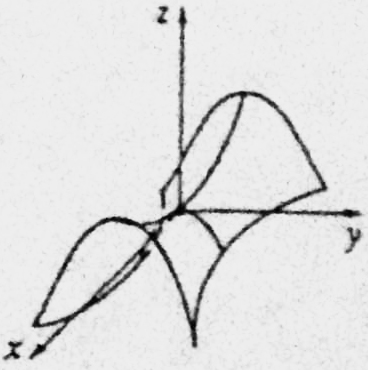
\includegraphics[height = 2cm]{Hyperbolic_paraboloid.jpg}   \\
	Parabolic Cylinder        & $x^2 = 4 a y$                                              & parabola             & $z$-axis             & $z$-axis              & 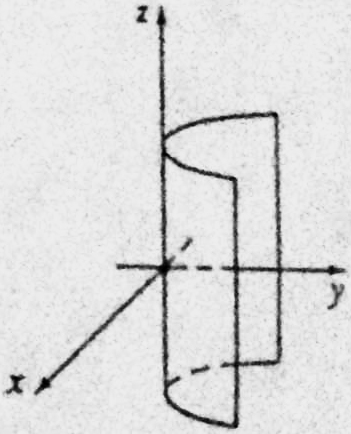
\includegraphics[height = 2cm]{Parabolic_cylinder.jpg}      \\
	Elliptic Cylinder         & $\frac{x^2}{a^2} + \frac{y^2}{b^2} = 1$                    & ellipse              & 2 parallel lines     & 2 parallel lines      & 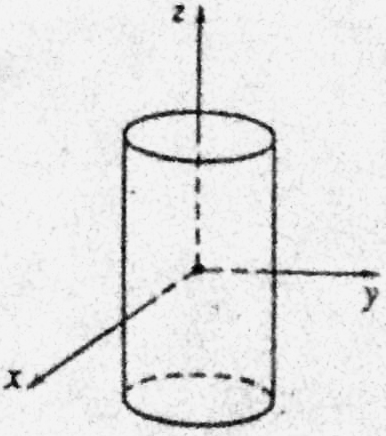
\includegraphics[height = 2cm]{Elliptic_cylinder.jpg}       \\
	Ellipsoid                 & $\frac{x^2}{a^2} + \frac{y^2}{b^2} + \frac{z^2}{c^2} = 1$  & ellipse              & ellipse              & ellipse               & 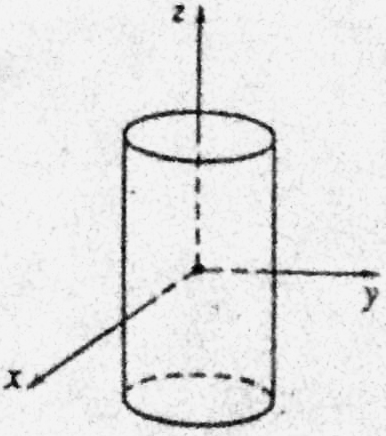
\includegraphics[height = 2cm]{Elliptic_cylinder.jpg}       \\
	\hline
\end{tabular}

\end{document}
